% !TeX program = pdflatex
% Expository summary of the current root V4 manuscript, 22 October 2026.
\documentclass[11pt,a4paper]{article}
\usepackage[T1]{fontenc}
\usepackage[utf8]{inputenc}
\usepackage{lmodern,microtype}
\usepackage{amsmath,amssymb,mathtools,mathrsfs}
\usepackage[a4paper,top=23mm,bottom=23mm,left=25mm,right=25mm,headheight=15pt]{geometry}
\usepackage{xcolor,booktabs,array,tabularx,enumitem,fancyhdr}
\usepackage{tikz}
\usetikzlibrary{arrows.meta}
\usepackage[hidelinks]{hyperref}
\definecolor{ink}{HTML}{123E48}
\definecolor{muted}{HTML}{52636B}
\definecolor{pale}{HTML}{EDF3F4}
\definecolor{markc}{HTML}{A33A2D}
\hypersetup{pdftitle={Pedagogical Summary of V4: Wilson Loops after the First Renormalisation Step},pdfauthor={},pdfsubject={Expository account of the V4 manuscript snapshot of 22 October 2026}}
\setlength{\parindent}{0pt}
\setlength{\parskip}{5.5pt}
\setlength{\emergencystretch}{2em}
\setlength{\abovedisplayskip}{9pt}
\setlength{\belowdisplayskip}{9pt}
\linespread{1.055}
\setlist[itemize]{leftmargin=1.4em,itemsep=3pt,topsep=3pt}
\setlist[enumerate]{leftmargin=1.6em,itemsep=3pt,topsep=3pt}
\pagestyle{fancy}
\fancyhf{}
\fancyhead[L]{\small\textcolor{muted}{Wilson Loops after the First RG Step}}
\fancyhead[R]{\small\textcolor{muted}{V4 Companion}}
\fancyfoot[C]{\small\thepage}
\renewcommand{\headrulewidth}{0.3pt}
\newcommand{\dd}{\mathrm{d}}
\newcommand{\Hol}{\operatorname{Hol}}
\newcommand{\tr}{\operatorname{tr}}
\newcommand{\id}{\mathbf 1}
\newcommand{\Eh}{\mathbb E_{\mathrm h}}
\newcommand{\Ph}{\mathbb P_{\mathrm h}}



\makeatletter % Stolen from the internet to make a fat \cdot which isn't as fat as a \bullet
\newcommand*{\bigcdot}{}% Check if undefined
\DeclareRobustCommand*{\bigcdot}{%
  \mathbin{\mathpalette\bigcdot@{}}%
}
\newcommand*{\bigcdot@scalefactor}{.7}
\newcommand*{\bigcdot@widthfactor}{1.15}
\newcommand*{\bigcdot@}[2]{%
  % #1: math style
  % #2: unused
  \sbox0{$#1\vcenter{}$}% math axis
  \sbox2{$#1\cdot\m@th$}%
  \hbox to \bigcdot@widthfactor\wd2{%
    \hfil
    \raise\ht0\hbox{%
      \scalebox{\bigcdot@scalefactor}{%
        \lower\ht0\hbox{$#1\bullet\m@th$}%
      }%
    }%
    \hfil
  }%
}
\makeatother






\newcommand{\chapterpage}[3]{\clearpage\phantomsection\label{summary:#1}\addcontentsline{toc}{section}{#1. #2}\noindent{\small\color{muted}#1\quad /\quad READING V4}\par\vspace{5pt}{\LARGE\bfseries\color{ink}#2\par}\vspace{5pt}{\footnotesize\color{muted}#3\par}\vspace{9pt}}
\newcommand{\subhead}[1]{\par\vspace{4pt}\textbf{\color{ink}#1}\par}
\newcommand{\idea}[1]{\begin{quote}\small\textbf{Key Idea.} #1\end{quote}}
\begin{document}
\thispagestyle{empty}
{\small\color{muted}PEDAGOGICAL COMPANION\hfill 22 OCTOBER 2026\par}
\vspace{23pt}
{\Huge\bfseries\color{ink}Wilson Loops after the First\\[5pt]Renormalisation Step\par}
\vspace{13pt}
{\LARGE A Pedagogical Summary of V4\par}
\vspace{15pt}
{\large From the Exact Lattice Integral to Scalar Extraction and Two-Loop Correlations\par}
\vspace{23pt}

V4 studies what happens to a Wilson loop insertion when the first layer of fine gauge-field fluctuations is integrated out. Its central achievement, as stated in the manuscript, is a quantitative first-step decomposition. A scalar contribution proportional to the length of the contour and a scalar contribution from its four corners are extracted. A Wilson loop insertion evaluated on the reconstructed background remains, together with explicitly controlled defect and boundary terms. V4 also treats the correlation function of two square loops with no common vertices, retaining their separate scalar factors and controlling additional contributions that connect them.

The organising formula says that the Wilson expectation is an extracted scalar times a retained expectation, plus a defect error and a boundary error.
Understanding this formula requires more than recognising a perimeter exponential. One must know which field occurs in the retained loop, which probability law averages it, how the coefficients are defined, and how the errors depend on contour length. Those questions organise this companion.

The intended reader knows basic Lie groups, Gaussian integration, and conditional expectation, but need not know Ba{\l}aban's renormalisation construction. Definitions are introduced before their estimates. The detailed combinatorics are explained through the role they play in the argument; the manuscript remains the source for their full proofs.

\subhead{The Scope of This Summary}
This account is based on the 22 October 2026 snapshot of \texttt{WILSON\_FIRST\_RG\_STEP\_V4.tex}. The discussion of dressed and ordinary coarse loops in Sections~3 and~24 includes the comparison added to V4 on 23 October; both source revisions are recorded in the source guide. Statements described as results are V4's stated results under its hypotheses, including its recorded readings of Ba{\l}aban. This companion adds no mathematical estimates and supplies no independent acceptance review. Separate continuation drafts are outside its scope.

The distinction between a fixed first step and an estimate that can be iterated is maintained throughout. V4's final section formulates an iteration conjecture and records the additional work it needs. Neither that conjecture nor a continuum limit follows merely from the existence of the first-step coefficients.

\vfill
{\small\color{muted}Base source revision: SHA-256 \texttt{D463C554B76F\ldots 73094E00}.\quad
    A detailed source guide appears on the last page.\par}

\clearpage
\thispagestyle{fancy}
\phantomsection\addcontentsline{toc}{section}{Reading Map}
{\LARGE\bfseries\color{ink}Reading Map\par}
\vspace{9pt}
The notation guide is on the next page. Read Sections 1--5 for the problem, the main result, and the physical law. Sections 6--16 explain the construction and scalar coefficients. Sections 17--24 explain the errors and retained insertion. Section 25 explains the two-loop extension. Sections 26--27 delimit iteration and locate the original arguments.

\vspace{5pt}
\begin{tabularx}{\textwidth}{@{}rXr@{}}
    \toprule
    & \textbf{Topic} & \textbf{Page}\\
    \midrule
    1 & The lattice, the action, and the observable & \pageref{summary:1}\\
    2 & Blocking as a transformation of measures & \pageref{summary:2}\\
    3 & The main result in readable form & \pageref{summary:3}\\
    4 & Hypotheses, scales, and uniformity & \pageref{summary:4}\\
    5 & Branches and the inherited physical law & \pageref{summary:5}\\
    6 & Solving the nonlinear block constraint & \pageref{summary:6}\\
    7 & The conditional integral and its exterior & \pageref{summary:7}\\
    8 & How local interactions become polymers & \pageref{summary:8}\\
    9 & Marking a closed nonabelian source & \pageref{summary:9}\\
    10 & Extracting the scalar inside the expansion & \pageref{summary:10}\\
    11 & The exact flat reference integral & \pageref{summary:11}\\
    12 & Gaussian marginals and hard cutoffs & \pageref{summary:12}\\
    13 & Connected logarithms and spatial decay & \pageref{summary:13}\\
    14 & The perimeter coefficient & \pageref{summary:14}\\
    15 & The corner coefficient & \pageref{summary:15}\\
    16 & Returning to a conditional region & \pageref{summary:16}\\
    17 & Exterior response as a covariance & \pageref{summary:17}\\
    18 & Paying bad regions with physical witnesses & \pageref{summary:18}\\
    19 & The signed integrated defect & \pageref{summary:19}\\
    20 & Why the integration region retreats & \pageref{summary:20}\\
    21 & Labelled sums and the second-order rate & \pageref{summary:21}\\
    22 & Averaging the finite-geometry exponent & \pageref{summary:22}\\
    23 & The size of the leading term at a fixed loop & \pageref{summary:23}\\
    24 & The outgoing insertion and closed flux factors & \pageref{summary:24}\\
    25 & Two disjoint square loops & \pageref{summary:25}\\
    26 & What iteration would still require & \pageref{summary:26}\\
    27 & Source guide and essential distinctions & \pageref{summary:27}\\
    \bottomrule
\end{tabularx}

\vspace{10pt}
\subhead{The Argument in One Chain}
\begin{center}
    \begin{tabular}{c}
        Exact blocking and the physical denominator\\
        $\downarrow$\\
        Conditional integral, closed marked groups, and scalar extraction\\
        $\downarrow$\\
        Flat line and corner coefficients, then regional identification\\
        $\downarrow$\\
        Signed defects, exterior response, and physical history averages
    \end{tabular}
\end{center}
The arrows indicate dependencies in the explanation. They do not mean that an estimate at a reference field automatically transfers to the interacting physical law.

\clearpage
\phantomsection\addcontentsline{toc}{section}{Notation at a Glance}
{\LARGE\bfseries\color{ink}Notation at a Glance\par}
\vspace{8pt}
The same letter can have different roles in different reference constructions. The following guide identifies the main objects; each is defined more fully when it enters the exposition.

\subhead{Fields, Geometry, and Operators}
\begin{small}
    \begin{tabularx}{\textwidth}{@{}p{0.24\textwidth}X@{}}
        \toprule
        \textbf{Symbol} & \textbf{Meaning}\\
        \midrule
        $G$, $\chi$ & Gauge group and normalised irreducible character.\\[3pt]
        $g_0$, $g_1$ & Bare coupling and first-step coupling.\\[3pt]
        $\varepsilon$, $L$ & Fine lattice spacing and blocking factor.\\[3pt]
        $U$, $V$, $U_1$ & Fine field, coarse field, and constrained fine background.\\[3pt]
        $C_n$, $n_C$ & Square of side $nL$ fine bonds; $n_C=4nL$ traversals.\\[3pt]
        $P(C_n)$ & Physical perimeter, $4nL\varepsilon$.\\[3pt]
        $I$, $J$, $D$ & Inner free carrier, exterior free carrier, and a general conditional free carrier.\\[3pt]
        $\mathsf C_U$, $h_U$ & $\mathsf C_UB$ is the element of $\ker LQ_U$ equal to $B$ on the free bonds; $h_U$ is the right inverse of $LQ_U$ supported on the designated bonds.\\[3pt]
        $H$, $\mathsf H$ & Conditional precision and flat free precision, respectively.\\[3pt]
        $C_T$, $\mathsf K_B$ & Flat free covariance; the names belong to different sections of V4.\\[3pt]
        $\mathsf K$ & Covariance after reconstructing the linear fine field.\\
        \bottomrule
    \end{tabularx}
\end{small}

\subhead{Laws, Extracted Scalars, and Errors}
\begin{small}
    \begin{tabularx}{\textwidth}{@{}p{0.24\textwidth}X@{}}
        \toprule
        $\rho_0$, $\mathcal Z_0$ & Bare density and its physical partition function.\\[3pt]
        $\rho_1$, $N_1$, $W_1$ & Blocked vacuum measure, observable numerator, and their Radon--Nikod\'{y}m quotient.\\[3pt]
        $\xi$, $\Eh$ & Branch data and its normalised physical history expectation.\\[3pt]
        $K_{\xi;t}$, $\nu_{\xi;t}$ & Interpolated conditional kernSSel and its normalised law.\\[3pt]
        $A_{\mathrm{cov}}$ & Event that the conditional carrier covers the loop's reconstruction inputs.\\[3pt]
        $S^\circ_{D,C,T}$ & Conditional flat reference scalar at carrier $D$.\\[3pt]
        $\kappa_v$, $\kappa_C$ & Straight-line logarithmic density and extracted square scalar; distinct uses of $\kappa$.\\[3pt]
        $\delta m$, $z_{\mathrm c}$ & Perimeter coefficient and square corner factor with the fixed cutoff convention.\\[3pt]
        $r$, $\tau$, $\rho$ & Fluctuation cutoff radius, forest-expansion parameter, and signed-source gain.\\[3pt]
        $\varepsilon_1$, $\pi_*$ & Small-field tolerance and the scale governing rare-witness tails.\\[3pt]
        $E^\circ$, $E_{\mathrm{def}}$, $E_{\mathrm{bdry}}$ & Finite-geometry exponent, signed defect, and boundary/uncovered error.\\
        \bottomrule
    \end{tabularx}
\end{small}

A \emph{carrier} is the set of variable labels on which an object lives. A \emph{mark} records a source contact or a specified bad event. A \emph{history} here includes the region choices and retained fields of this first step; it need not represent several RG scales.

\chapterpage{1}{The Lattice, the Action, and the Observable}{V4, Section 1; equations defining the Wilson insertion and the bare action.}

The starting point is a four-dimensional periodic lattice with fine spacing $\varepsilon$. A positive oriented bond $b$ carries a group element $U(b)$ in a compact connected simple Lie group $G\subset U(N)$. The value on the reversed bond is $U(b^{-1})=U(b)^{-1}$. The finite torus makes every original integral finite-dimensional. The size of the torus remains a parameter in the estimates.

For an ordered closed contour $C=(b_1,\ldots,b_{n_C})$, V4 uses
\begin{equation*}
    \Hol_U C=U(b_1)\cdots U(b_{n_C})\;,
    \qquad W_\chi(C;U)=\chi(\Hol_U C)\;.
\end{equation*}
Here $\chi$ is an irreducible character divided by the dimension of its representation, so $\chi(\id)=1$ and $|\chi(g)|\leqslant  1$. The order of the factors matters: generally, gauge-group elements do not commute.

A site gauge transformation acts on a bond by changing the frames at its two endpoints. Around a closed contour the intermediate frame changes cancel. The holonomy is conjugated at the base point, and the character is unchanged. Thus the Wilson loop insertion is a gauge-invariant function of the field. This invariance must survive the later localisation and expansion.

With $\tr_N \coloneqq N^{-1}\operatorname{Tr}$, the action and its density are
\begin{equation*}
    S(U) \coloneqq \sum_{p\in \mathcal P_T} \bigl(1-\operatorname{Re}\tr_N U(\partial p)\bigr)\;,
    \qquad \rho_0(U) \coloneqq e^{-g_0^{-2}S(U)-E_\varepsilon}\;.
\end{equation*}
The sum is over unoriented plaquettes, each counted once and $E_\varepsilon$ is Ba{\l}aban's vacuum renormalisation. Product normalised Haar measure is denoted by $\dd U$. The bare expectation is
\begin{equation*}
    \mathbb E_\varepsilon[W_\chi(C)]
    =\frac{\int W_\chi(C;U)\rho_0(U)\,\dd U}
        {\int\rho_0(U)\,\dd U}\;.
\end{equation*}

The contour of the main theorem is a square $C_n$ of with $nL$ find bonds along each side. It has $n_C=4nL$ fine bonds, $4n$ coarse segments, and physical perimeter $P(C_n)=4nL\varepsilon$. Each coarse segment contains $L$ fine bonds. These three ways of measuring size must be kept distinct when interpreting a perimeter rate.

\idea{The observable is closed from the beginning. Its gauge invariance is a structural input to the proof, not an operation performed after estimating separate pieces of the contour.}

\chapterpage{2}{Blocking as a Transformation of Measures}{V4, Section 1, ``Normalisation'', and Section 8, ``The Numerator Carried to the Next Transformation''.}

Blocking assigns a coarse field $V$ to a fine field $U$ through a Borel map $M$. On a regular logarithm domain, $M$ is Ba{\l}aban's nonlinear group average. V4 chooses a Borel, gauge-covariant extension to all fine configurations, using the straight fine transport wherever the logarithmic formula is unavailable. This extension makes the unrestricted blocking operation a defined, gauge-covariant map on the entire configuration space.

In the notation of the manuscript, the blocking kernel is defined to be
\begin{equation*}
    (T\rho)(V) \coloneqq \int
        \prod_{c\in E_1}\delta_G\bigl(M(U,c)V(c)^{-1}\bigr)
        \rho(U)\,\dd U\;.
\end{equation*}
The group Dirac measure is normalised against Haar measure. The clean measure-theoretic interpretation of $T$ is a pushforward of the measure $\rho(U) \, \dd  U$ under $M$. It remains meaningful even when a density with respect to coarse Haar measure has not been specified.

Two measures are transformed together:
\begin{equation*}
    \rho_1=M_*(\rho_0\,\dd U)\;,
    \qquad N_1=M_*(W_\chi(C;\,\bigcdot\,)\rho_0\,\dd U)\;.
\end{equation*}
The first is positive; the second can be complex. Positivity of the kernel and $|W_\chi|\leqslant  1$ give $|N_1|\leqslant  \rho_1$, where $|N_1|$ denotes the total variation of $N_1$. Hence, the outgoing insertion exists as a Radon--Nikod\'{y}m derivative. For $\rho_1$-almost every $V$,
\begin{equation*}
    W_1(C;V)=\frac{\dd N_1}{\dd\rho_1}(V)\;,
    \qquad |W_1(C;V)|\leqslant  1\;.
\end{equation*}
Equivalently, it is the conditional expectation of the original Wilson loop insertion given the coarse field. This is an exact description of the observable after blocking, before any perimeter extraction.

The physical normalisation is preserved:
\begin{equation*}
    \mathcal Z_0=\int\rho_0(U)\,\dd U
        =\rho_1(G^{E_1})>0\;,
    \qquad
    \mathbb E_\varepsilon[W_\chi(C)]
        =\mathcal Z_0^{-1}\int W_1(C;V)\,\dd\rho_1(V)\;.
\end{equation*}
Later conditional fluctuation integrals have their own normalising factors. They occur inside the construction of $N_1$ and $\rho_1$; they do not replace $\mathcal Z_0$.

\idea{A renormalisation step transports both the observable numerator and the vacuum measure. An estimate of the transported numerator becomes a physical expectation estimate only with the same denominator retained.}

\chapterpage{3}{The Main Result in Readable Form}{V4, Theorem 1.2; the proposition ``the leading term and the coarse loop''; Appendix F.}

The single-loop theorem extracts a scalar factor from the expectation of a leading coarse insertion, with two error terms. Under V4's hypotheses (H1)--(H4), it states
\begin{equation*}
        \mathbb E_\varepsilon[W_\chi(C_n; \, \bigcdot \, )] =\kappa_{C_n}\, \int W^1_{\chi}(C_n;V) \, \dd \rho_1(V)/\mathcal Z_0  +E_{\mathrm{def}}+E_{\mathrm{bdry}}\;,
\end{equation*}
where, for $\rho_1$-almost every $V$,
\begin{equation*}
    W^1_{\chi}(C;V)\coloneqq \Eh\!\left[\id_{A_{\mathrm{cov}}}
        e^{E^\circ_\xi}W_\chi(C;U_1(V,V_0))
        \,\middle|\,V\right]\;,
    \quad
    \kappa_{C_n}
        =e^{-\delta m(g_0,\varepsilon)P(C_n)}
            \bigl(z_{\mathrm c}(g_0,\pi/2)\bigr)^4
        \neq 0\;.
\end{equation*}
We fix an adjoint-invariant norm $|\cdot|$ on the Lie algebra $\mathfrak g$. Dependence on this norm and the fixed cutoff conventions is left implicit.

\subhead{What the Factors Mean}
The perimeter coefficient $\delta m$ comes from the connected density along an infinite straight reference contour. The corner factor $z_{\mathrm c}$ subtracts the two straight densities from a bent reference contour. Both are defined by convergent connected sums in the same normalised reference integral; see Sections~\hyperref[summary:14]{14}--\hyperref[summary:15]{15}.

$U$ is the original fine field. The field $U_1(V,V_0)$ is also fine, it is the constrained background determined by the coarse field $V$ and exterior fine field $V_0$. It satisfies $M(U_1)=V$ on the constrained regular bonds. Both loops follow the fine contour $C_n$. The conditional expectation averages exterior fields and region choices at fixed $V$. The indicator $\id_{A_{\mathrm{cov}}}$ selects the terms in which fine fluctuations along the loop can be expanded to extract the perimeter and corner factors carrying the expected ultraviolet divergences. Section~\hyperref[summary:16]{16} explains the coverage condition that makes this extraction possible. Terms outside $A_{\mathrm{cov}}$ are included in $E_{\mathrm{bdry}}$ and controlled using large-field probabilities, as explained in Section~\hyperref[summary:18]{18}. The exponent $E^\circ_\xi$ records the boundary, torus, and distant-corner corrections, whose accumulated effect on the renormalised loop expectation is expected to remain bounded as the ultraviolet cutoff is removed.

The leading $W^1_\chi$ differs from the exact outgoing $W_1=\dd N_1/\dd\rho_1$ of Section~2. The absolute expectation errors $E_{\mathrm{def}}$ and $E_{\mathrm{bdry}}$ account for the signed defect in scalar extraction and the exterior response or uncovered configurations, respectively.

\subhead{Dressed Versus Ordinary Coarse Loops}
An ordinary (or na{\"i}ve) coarse loop multiplies $V(c)$ around the blocked contour. Nonlinear blocking need not make $V(c)$ equal to the straight fine transport in $U_1$. Rewriting the background loop in coarse links therefore leaves additional field-dependent factors inside the closed character. Together with the regional weights, these remain in $W^1_\chi$: it is a dressed Wilson loop.

V4's pointwise comparison of the background loop with the ordinary coarse loop, on covered configurations, costs schematically order $g_0$ per coarse contour bond, up to logarithms. At fixed physical perimeter the number of bonds grows like $\varepsilon^{-1}$. We therefore aim to retain the dressed insertion through further RG steps and postpone comparison with an ordinary loop until a fixed final coarse scale.

\idea{The RG transforms the observable as well as the measure. Extracting scalar factors leaves a dressed insertion whose iteration still needs to be proved.}


\chapterpage{4}{Hypotheses, Scales, and Uniformity}{V4, hypotheses (H1)--(H4), Theorem 1.2(ii)--(iii), Appendix B, ``The thresholds''.}

\subhead{The Order of Choices}
V4 fixes its parameters in a strict order, and every constant may depend only on the choices made before it:
\begin{equation*}
    \underbrace{G,\ \chi,\ L,\ \text{constants}}_{\text{(H1)},\ L>11\text{ odd}}
    \;\longrightarrow\;
    \underbrace{0<g_0<g_*}_{\text{(H2)}}
    \;\longrightarrow\;
    \underbrace{\text{torus, large}}_{\text{(H3)}}\;.
\end{equation*}
In particular every constant below is independent of $g_0$, the loop size $n$, the torus, and the history.

\subhead{The Scales}
As $g_0\to0$,
\begin{equation*}
    \begin{aligned}
        r&=A_1(\log g_0^{-2})^{p_0}\to\infty\;, &&\text{the cutoff radius of the rescaled fluctuation }A/g_0\;,\\
        \tau&=C\bigl[g_0(1+r)^3+e^{-cr^2}\bigr]\to0\;, &&\text{the cluster-expansion parameter}\;,\\
        \pi_*&\to\infty\;, &&\text{the large-field scale}\;,\\
        \varepsilon_1&\to0\;, &&\text{the coarse small-field tolerance}\;.
    \end{aligned}
\end{equation*}
Up to powers of $\log g_0^{-2}$, both $\tau$ and $\varepsilon_1$ are of order $g_0$, while $e^{-c\pi_*^2}$ vanishes faster than every power of $g_0$. The signed-source gain $\rho=O(g_0^2(1+r)^4)$ is explained in Section~\hyperref[summary:10]{10}.

\subhead{The Bounds}
Let $n_C=4nL$ be the number of contour bonds, and let $d_j$, $\iota_T$ be the distances of Section~\hyperref[summary:16]{16}. On covered branches V4 states
\begin{equation*}
    |E^\circ_\xi|\leqslant C\tau^2\Bigl[\sum_{j=0}^{4n-1}e^{-cd_j}+4ne^{-c\iota_T}+(n+1)e^{-cn}\Bigr]\leqslant C\tau^2(9n+1)\;,
\end{equation*}
and for the physical errors
\begin{equation*}
    \begin{aligned}
        |E_{\mathrm{def}}|
        &\leqslant C'_Ln_Ce^{-(c_*/2)\pi_*^2}+e^{C_\chi n_C\rho(\varepsilon_1+e^{-cb/(LM)})}-1\;,\\
        |E_{\mathrm{bdry}}|
        &\leqslant C_{\mathrm{resp},\chi}\,n_C(1+g_0r)\,e^{-c_*\pi_*^2}\;,
    \end{aligned}
\end{equation*}
where $e^{-cb/(LM)}$ vanishes faster than every power of $g_0$. At fixed $n$, every error therefore vanishes faster than every power of $g_0$ except the second term of $E_{\mathrm{def}}$, which is of order $n_C\rho\varepsilon_1$ when that is small. The factors $n_C$ are explicit; they are not absorbed into the constants.

Hypothesis (H4) takes Ba{\l}aban's results as stated, together with V4's readings of conventions his papers leave implicit.

\idea{Uniform constants and uniform smallness are different. A bound can have constants independent of $g_0$, $n$, and the torus while growing exponentially with the number $n_C$ of contour bonds.}




\chapterpage{5}{Branches and the Inherited Physical Law}{V4, Section 3.1; Appendix D, ``The physical substitution''.}

Theorem~1.2 states its leading term as an expectation $\Eh$ over branch data $\xi$, listed at the end of this section. The whole section explains one identity:
\begin{equation*}
    \mathbb E_\varepsilon[W_\chi(C)]=\Eh\Bigl[\int W_\chi(C;U_\xi(a))\,\dd\nu_{\xi;1}(a)\Bigr]\;.
\end{equation*}
It splits the bare expectation into two levels. Inside, the branch data $\xi$ is fixed and only a small fluctuation $a$ is integrated, against a normalised law $\nu_{\xi;1}$ (Section~\hyperref[summary:7]{7}); Sections~\hyperref[summary:6]{6}--\hyperref[summary:17]{17} work at this level, with bounds uniform in $\xi$. Outside, $\Eh$ averages over $\xi$; from Section~\hyperref[summary:18]{18} on, the fixed-$\xi$ results are averaged, and the branches with a bad region near the loop are paid for by their small $\Eh$-probabilities.

\subhead{The Outer Law}
At fixed $\xi$ the integral over $a$ has a density $\mathcal K_\xi$ with mass $\mathsf w_\xi=\int\mathcal K_\xi(a)\,\dd a$, so that $\nu_{\xi;1}=\mathsf w_\xi^{-1}\mathcal K_\xi\,\dd a$. Writing $\mathcal O$ for the remaining sums and integrals over the branch data, with Ba{\l}aban's large-field factors, constraints, Jacobians, and the background action $e^{-g_0^{-2}S(U_1)}$, the history expectation is
\begin{equation*}
    \Eh[X]=\frac{1}{\mathcal Z_0}\int\mathcal O[\mathsf w_\xi X](V)\,\dd V\;,\qquad \Eh[1]=1\;.
\end{equation*}
$\mathcal O$ is the outer part of Ba{\l}aban's formula for the blocked density \cite[eq.~(1.15)]{BalabanCRE}, everything except the integral over the small fluctuations, after his splitting (1.18) and change of variables (1.22). The law $\Eh$ is not a reference measure chosen for convenience. It is built from the same interacting integral and normalised by the physical partition function $\mathcal Z_0$.

\subhead{The Branch Data}
Ba{\l}aban's first step inserts partitions of unity into the fine integral, one factor per cube, each testing whether a field is small or large there \cite[pp.~245--251]{BalabanCRE}. Expanding the products rewrites the integral as a sum of terms, the \emph{branches}, each labelled by
\begin{equation*}
    \xi=(\Omega_1,R_1,V,V_0,A_{\mathrm e})\;.
\end{equation*}
Here
\begin{itemize}
    \item $\Omega_1$ is the small-field region \cite[eq.~(1.10)]{BalabanCRE};
    \item $R_1\subset\Omega_1$ is the large-fluctuation region, the union of the cubes on which some fluctuation reaches the cutoff radius, $|A(b)|\geqslant r$ \cite[eq.~(1.18)]{BalabanCRE};
    \item $V$ is the coarse field;
    \item $V_0$ is the fine field on the bonds outside $\Omega_1$; and
    \item $A_{\mathrm e}$ is the exterior fluctuation, on the free bonds of $\Omega_1$ outside $\Lambda_1$ (see below).
\end{itemize}
From $\Omega_1$ and $R_1$ Ba{\l}aban builds the final small-field domain \cite[eq.~(1.20)]{BalabanCRE}:
\begin{equation*}
    \Lambda_1\subset\Omega_1\setminus R_1\;,
\end{equation*}
separated from the boundary of $\Omega_1$ and from $R_1$ by collars of cubes of side $LMR_1$. At fixed branch data only the fluctuation $a$ on the \emph{free} bonds $I$ of $\Lambda_1$ (see Section~\hyperref[summary:6]{6}) is integrated; $A_{\mathrm e}$ is the fluctuation on the remaining free bonds $J$ of $\Omega_1$. Together, $a$ and the branch data determine the fine field $U_\xi(a)$.

Ba{\l}aban fixes an axial gauge inside each block, which adds a term $\mathbf G(U)$ to the action \cite[eqs.~(1.5)--(1.7)]{BalabanCRE}; without it, gauge transformations trivial at the block centres would be zero modes of the Hessian. The background $U_1$ minimises the action plus $\mathbf G$ with block average $V$ and $U_1=V_0$ off $\Omega_1$ \cite[eq.~(1.12)]{BalabanCRE}.

\idea{Conditioning freezes variables but does not make them independent or harmless. Their distribution and every remaining normaliser are inherited from the same interacting integral.}


\chapterpage{6b}{Solving the Nonlinear Block Constraint}{V4, Sections 3.2--3.3; Appendix B.}
\label{summary:6}

At fixed branch data the fluctuation integral is \cite[eq.~(1.11)]{BalabanCRE}
\begin{equation*}
    \int W_\chi(C;U)\,(\text{cutoff factors})\,\delta\bigl(\mathsf M(U)V^{-1}\bigr)\,e^{-g_0^{-2}(S+\mathbf G)(U)}\,\dd U\;,
\end{equation*}
an integral over the fine bonds of $\Omega_1$ with Haar measure and one $\delta$-function for each coarse bond $c$, which forces the block averages to equal $V$. The cluster expansion of Section~\hyperref[summary:8]{8} needs a Gaussian integral over a vector space with small local corrections instead. Four steps produce it.

\subhead{Coordinates}
We write a fine field near the minimising background $U_1$ as $U=e^{iq}U_1$, with $q$ a $\mathfrak g$-valued phase on the fine bonds of $\Omega_1$ \cite[eq.~(1.13)]{BalabanCRE}. The Haar measure becomes $\sigma(q)\,\dd q$, and the constraint enforced by the $\delta$-function becomes $\mathcal Q_{U_1}(q)=0$, one equation in $\mathfrak g$ for each $c$:
\begin{equation*}
    \mathcal Q_{U_1}(q)=\frac{1}{i}\log\bigl(\mathsf M(e^{iq}U_1)V^{-1}\bigr)=LQ_{U_1}q+\mathcal N_{U_1}(q)\;,
\end{equation*}
with $LQ_{U_1}$ linear, Lemmata 3.2 and B.8 of V4 show surjectivity, and $\mathcal N_{U_1}$ quadratic at $q=0$. The constraint is nonlinear, so the phases that satisfy it form a curved set.

\subhead{Linearisation}
For each $c$ one fine bond $b_0(c)$ is \emph{designated}; the other bonds are \emph{free} \cite[p.~249]{BalabanCRE}. Let $h_{U_1}$ be the right inverse of $LQ_{U_1}$ supported on the designated bonds, and let $\widetilde D_{U_1}(A)$ be the small solution of
\begin{equation*}
    \widetilde D_{U_1}(A)=\mathcal N_{U_1}\bigl(A-h_{U_1}\widetilde D_{U_1}(A)\bigr)\;.
\end{equation*}
Then $\mathcal Q_{U_1}\bigl(A-h_{U_1}\widetilde D_{U_1}(A)\bigr)=LQ_{U_1}A$ for every $A$. The substitution $q=A-h_{U_1}\widetilde D_{U_1}(A)$, which moves only the designated bonds, therefore turns the constraint into the linear constraint $LQ_{U_1}A=0$ \cite[eq.~(1.14)]{BalabanCRE}. Its Jacobian becomes a term of the exponent.

\subhead{Solution}
The linear constraint fixes $A$ on the designated bonds as a linear function of $A$ on the free bonds. With the free variables scaled by $g_0$,
\begin{equation*}
    A=g_0\mathsf C_{U_1}B\;,\qquad q_{U_1}(B)\coloneqq A-h_{U_1}\widetilde D_{U_1}(A)\;,
\end{equation*}
where $\mathsf C_{U_1}B$ is the unique element of $\ker LQ_{U_1}$ that agrees with $B$ on the free bonds. Integrating the $\delta$-functions against the designated variables gives a constant, and the field $B$ on the free bonds is unconstrained.

\subhead{Expansion}
The action at $e^{iq_{U_1}(B)}U_1$ has no linear term in $B$, since $U_1$ minimises it under the block constraint \cite[eq.~(1.12)]{BalabanCRE}. Up to constants, the result is \cite[eq.~(1.15)]{BalabanCRE}
\begin{equation*}
    \int W_\chi\bigl(C;e^{iq_{U_1}(B)}U_1\bigr)\,(\text{cutoff factors})\exp\Bigl(-\tfrac12\langle B,H_\xi B\rangle+\sum_{\mathfrak p}\mathfrak p(B)\Bigr)\,\dd B\;,
\end{equation*}
where $\tfrac12\langle B,H_\xi B\rangle$ is the quadratic part of the action plus gauge fixing, and the $\mathfrak p$ are local terms: the rest of the action and gauge fixing, the Haar density, and the Jacobian (Section~\hyperref[summary:8]{8}). They depend on $B$ only via $g_{0} \mathsf{C}_{U_1}B$.

This is the integral that the rest of the summary expands. At the identity background $H_\xi$ is the form $\mathsf H$ of Section~\hyperref[summary:11]{11}. Two further properties are used later.
\begin{itemize}
    \item \emph{Locality.} The equation for $c$ involves only the two blocks at the ends of $c$ and only its own designated bond. Each designated phase therefore depends on a fixed finite set of free bonds, its \emph{stencil}, and the terms of the exponent are local (Sections~\hyperref[summary:8]{8}, \hyperref[summary:9]{9}, and \hyperref[summary:16]{16}).
    \item \emph{The Quadratic Correction.} Since $\widetilde D_{U_1}(A)=O(|A|^2)$ and $|A|\lesssim g_0r$, the non-Gaussian part of $g_0^{-2}S$ starts at cubic order and is $O(g_0(1+r)^3)$. This is the first term of $\tau$ (Section~\hyperref[summary:4]{4}).
\end{itemize}
V4 proves that the substitution is unique and analytic, with a nonvanishing Jacobian, on the whole cutoff region and not only near $q=0$; this takes up most of Appendix~B.

\idea{A change of variables on one designated bond per coarse bond makes the block constraint linear, and the linear constraint is then solved exactly. The result is a Gaussian integral over the free bonds with local corrections that start at cubic order.}


\chapterpage{7}{The Conditional Integral and Its Exterior}{V4, Section 3.4, ``The boundary law, the exterior interpolation and the collar''.}

In the integral of Section~\hyperref[summary:6]{6}, the cutoff factors on $R_1$ and near the boundary of $\Omega_1$ test the field $e^{iq}U_1$, and $U_1$ depends on the coarse field $V$ on all of $\Omega_1$, including $\Lambda_1$. The next renormalisation step needs these factors to depend on $V$ only outside $\Lambda_1$. Ba{\l}aban therefore replaces $U_1$ in them by a background determined by $V$ outside $\Lambda_1$ alone, which differs from $U_1$ there by an exponentially small amount, and absorbs the difference into a small shift $\Psi_\xi$ of the fluctuation variables on those bonds \cite[eqs.~(1.21)--(1.22)]{BalabanCRE}. 

The free field can therefore be written as $B=\Psi_\xi(a+A_{\mathrm e})$, where the fluctuation $a\in\mathfrak g^I$ is integrated and the exterior fluctuation $A_{\mathrm e}\in\mathfrak g^J$ is held fixed. The shift $\Psi_\xi$ acts bond by bond and only on a strip far from $I$, so near $I$ the phase is simply $q_{U_1}(a+A_{\mathrm e})$. The fine field is
\begin{equation*}
    U_\xi(a)=e^{iq_{U_1}(\Psi_\xi(a+A_{\mathrm e}))}U_1\quad\text{on }\Omega_1\;,\qquad U_\xi(a)=V_0\quad\text{off }\Omega_1\;,
\end{equation*}
and $\mathcal K_\xi$ is a density on $\mathfrak g^I$.

The exterior field enters the integrand in two ways: through the off-diagonal block of the quadratic form, and through the local terms of the exponent whose stencils meet both $I$ and $J$. V4 switches both off with a parameter $0\leqslant t\leqslant1$:
\begin{equation*}
    K_{\xi;t}(a)=\id_{\mathcal D_I}(a)\exp\Bigl(-\tfrac12\langle a,H_{\xi,II}a\rangle-t\langle a,H_{\xi,IJ}A_{\mathrm e}\rangle+P_{\xi,t}(a)\Bigr)\;,\quad \dd\nu_{\xi;t}(a)=\frac{K_{\xi;t}(a)\,\dd a}{\int K_{\xi;t}(a')\,\dd a'}\;.
\end{equation*}
Here $H_\xi$ is the quadratic form of Section~\hyperref[summary:6]{6}, with blocks $H_{\xi,II}$ and $H_{\xi,IJ}$; $\mathcal D_I=\{a\,|\,|a(b)|<r\text{ for all }b\in I\}$ is the hard cutoff; and $P_{\xi,t}(a)$ is the sum of the local terms of the exponent near $I$, evaluated at $a+tA_{\mathrm e}$, defined in Section~\hyperref[summary:8]{8}.
\begin{itemize}
    \item At $t=1$ this is the actual conditional law: $\mathcal K_\xi=e^{c_\xi}K_{\xi;1}$, where the constant $c_\xi$ collects every term that does not depend on $a$. Hence $\nu_{\xi;1}$ is the law of Section~\hyperref[summary:5]{5}.
    \item At $t=0$ the exterior field is switched off. The centred law $\nu_{\xi;0}$ has no linear term, and Sections~\hyperref[summary:8]{8}--\hyperref[summary:16]{16} expand it into polymers.
\end{itemize}

The Wilson function is not interpolated: for every $t$ it is $W_\chi(C;U_\xi(a))$ at the actual $A_{\mathrm e}$. Let $F_\xi(t)=\int W_\chi(C;U_\xi(a))\,\dd\nu_{\xi;t}(a)$. Since the normaliser of $\nu_{\xi;t}$ also depends on $t$, differentiating gives a covariance:
\begin{equation*}
    F_\xi(1)=F_\xi(0)+\mathcal B_\xi\;,\qquad \mathcal B_\xi=\int_0^1\operatorname{Cov}_{\nu_{\xi;t}}\bigl(W_\chi(C;U_\xi(a)),\,\partial_t\log K_{\xi;t}(a)\bigr)\,\dd t\;.
\end{equation*}
The exterior response $\mathcal B_\xi$ is bounded in Section~\hyperref[summary:17]{17}. The hard cutoff $\mathcal D_I$ is the same for every $t$.

\idea{The exterior enters the conditional law only through a linear coupling and the local terms at the edge of $I$. Switching them off gives a centred law for the expansion, and the difference is a covariance that is bounded separately.}


\chapterpage{8}{How Local Interactions Become Polymers}{V4, Sections 3.3, 3.5--3.6; Appendix B, activity and vacuum-cluster bounds.}

With $H=H_{\xi,II}$ and $\chi_b(a)=\id_{\{|a(b)|<r\}}$, the centred kernel of Section~\hyperref[summary:7]{7} is
\begin{equation*}
    K_{\xi;0}(a)=\prod_{b\in I}\chi_b(a)\,e^{-\frac12\langle a,Ha\rangle+P_{\xi,0}(a)}\;,
\end{equation*}
a Gaussian times a local perturbation and a hard cutoff. To obtain bounds that do not depend on the volume, V4 writes its integral as a \emph{polymer gas}: a sum over families of disjoint connected regions, each carrying a small weight. This is Ba{\l}aban's cluster expansion \cite[Sect.~2]{BalabanRG2}.

\subhead{The Local Terms}
As a function of the free field $B$, the exponent of the integral over the fluctuation $A$ on $\Omega_1$ in Ba{\l}aban's formula for the blocked density \cite[eq.~(1.15)]{BalabanCRE} is, up to a constant,
\begin{equation*}
    -\tfrac12\langle B,H_\xi B\rangle+\sum_{\mathfrak p}\mathfrak p(B)\;.
\end{equation*}
There is no linear term, because $U_1$ minimises the action plus gauge fixing under the block constraint \cite[eq.~(1.12)]{BalabanCRE}. The $\mathfrak p$ are local terms of three kinds, each vanishing at $B=0$:
\begin{itemize}
    \item for each plaquette $p$, the action term $-g_0^{-2}\bigl[s_p(q_{U_1}(B))-s_p(0)\bigr]$, with $s_p(q)=1-\operatorname{Re}\tr\bigl((e^{iq}U_1)(\partial p)\bigr)$, minus its Taylor polynomial of degree two at $B=0$, and likewise for the gauge-fixing term of each block;
    \item for each bond $b$, the Haar term $\log\sigma(q_{U_1}(B)(b))-\log\sigma(0)$, where $\sigma(q)\,\dd q$ is the Haar measure in the coordinate $e^{iq}$;
    \item for each coarse bond $c$, the Jacobian term $\log\bigl|\det\bigl(\id-h_{U_1}(c)\,\partial_{A(b_0(c))}\widetilde D_{U_1,c}(A)\bigr)\bigr|$ of the substitution of Section~\hyperref[summary:6]{6}, at $A=g_0\mathsf C_{U_1}B$.
\end{itemize}
Each $\mathfrak p$ depends on $B$ only through the free bonds of a stencil. It is \emph{near} if this stencil meets $I$. The other terms depend only on $A_{\mathrm e}$ and the branch data and are constants at fixed $\xi$. The correction sum of Section~\hyperref[summary:7]{7} is
\begin{equation*}
    P_{\xi,t}(a) \coloneqq \sum_{\mathfrak p\ \mathrm{near}}\mathfrak p(a+tA_{\mathrm e})\;,\qquad 0\leqslant t\leqslant1\;.
\end{equation*}

\subhead{The Local Potentials}
Each near term $\mathfrak p$ is assigned a \emph{host} $Y$, a small connected union of $M$-cubes containing its stencil. The potential $\mathbf V_\xi(Y,a)$ is the sum of the values $\mathfrak p(a)$ of the near terms with host $Y$, so that
\begin{equation*}
    \sum_Y\mathbf V_\xi(Y,a)=P_{\xi,0}(a)\;,\qquad |\mathbf V_\xi(Y,a)|\leqslant Cg_0(1+r)^3\quad\text{on the cutoff box}\;.
\end{equation*}

\begin{figure}[ht]
\centering
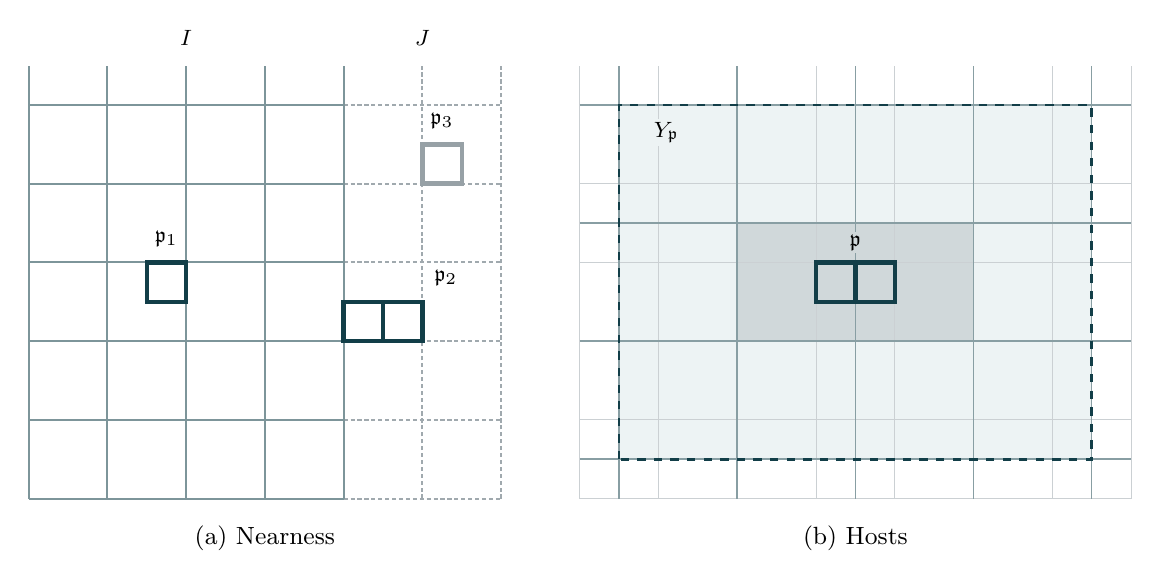
\begin{tikzpicture}[x=5mm, y=5mm,
    lat/.style={draw=muted!30, line width=0.3pt},
    term/.style={draw=ink, line width=1.6pt},
    lab/.style={font=\footnotesize, inner sep=1pt}]
    \draw[muted!55, line width=0.7pt, dash pattern=on 1.5pt off 1pt] (8,0) grid (12,11);
    \draw[ink!55, line width=0.7pt] (0,0) grid (8,11);
    \node[lab] at (4,11.7) {$I$};
    \node[lab] at (10,11.7) {$J$};
    \draw[term] (3,5) rectangle (4,6);
    \node[lab, fill=white] at (3.5,6.6) {$\mathfrak p_1$};
    \draw[term] (8,4) rectangle (10,5) (9,4) -- (9,5);
    \node[lab, fill=white] at (10.6,5.6) {$\mathfrak p_2$};
    \draw[term, draw=muted!60] (10,8) rectangle (11,9);
    \node[lab, fill=white] at (10.5,9.6) {$\mathfrak p_3$};
    \node[font=\small] at (6,-1) {(a) Nearness};

    \begin{scope}[shift={(14,0)}]
        \fill[pale] (1,1) rectangle (13,10);
        \fill[ink!20] (4,4) rectangle (10,7);
        \draw[lat] (0,0) grid (14,11);
        \foreach \x in {1,4,7,10,13} \draw[ink!50, line width=0.6pt] (\x,0) -- (\x,11);
        \foreach \y in {1,4,7,10} \draw[ink!50, line width=0.6pt] (0,\y) -- (14,\y);
        \draw[ink, dashed, line width=0.9pt] (1,1) rectangle (13,10);
        \draw[term] (6,5) rectangle (8,6) (7,5) -- (7,6);
        \node[lab, fill=ink!20] at (7,6.5) {$\mathfrak p$};
        \node[lab, fill=pale] at (2.2,9.3) {$Y_{\mathfrak p}$};
    \end{scope}
    \node[font=\small] at (21,-1) {(b) Hosts};
\end{tikzpicture}
\caption{(a) The bonds of $I$ are solid, and the bonds of $J$ are dashed. A local term is near when its stencil (thick) meets $I$. The terms $\mathfrak p_1$ and $\mathfrak p_2$ are near, and $\mathfrak p_2$ also reads exterior bonds, which is how $A_{\mathrm e}$ enters. The term $\mathfrak p_3$ is not near and is a constant at fixed $\xi$. (b) The thicker lines bound the $M$-cubes. The stencil of a near term $\mathfrak p$ meets the dark $M$-cubes. Its host $Y_{\mathfrak p}$ (dashed) is the smallest rectangle of $M$-cubes containing them, enlarged by one layer of cubes. The stencil is shorter than $M$, so it meets at most two cubes in each direction, and the host is at most four cubes wide. Selected hosts, bad bonds, and differentiated cubes make up the polymers.}
\end{figure}

\subhead{Three Expansions}
Each of the following steps is an exact identity.
\begin{itemize}
    \item \emph{Potentials.} Writing $e^{\mathbf V}=1+\int_0^1\mathbf Ve^{t\mathbf V}\,\dd t$ for every host selects a finite family of hosts \cite[eq.~(2.1)]{BalabanRG2}. Each selected host contributes a factor $\mathbf V$ of size $g_0(1+r)^3$.
    \item \emph{Cutoff.} Writing $\chi_b=1-(1-\chi_b)$ for every bond outside the selected hosts selects a set $\mathsf P$ of bad bonds, with sign $(-1)^{|\mathsf P|}$ \cite[eq.~(2.3)]{BalabanRG2}. A bad bond has $|a(b)|\geqslant r$, which costs $e^{-cr^2}$ under the Gaussian.
    \item \emph{Gaussian.} The covariance $H^{-1}$ couples all bonds. V4 writes $H^{-1/2}$ as a sum over walks with finite-range steps and attaches to every coarse cube $\Delta$ a parameter $s_\Delta\in[0,1]$ that switches off the walks entering $\Delta$. Writing the value at $s_\Delta=1$ as the value at $s_\Delta=0$ plus $\int_0^1\partial_{s_\Delta}\,\dd s_\Delta$ selects the cubes on which the coupling is kept \cite[eq.~(2.8)]{BalabanRG2}. Each such cube costs a decay factor of the walk series.
\end{itemize}
The selected hosts, the bad bonds, and the differentiated cubes form a \emph{final domain} $Z$, a union of coarse cubes. After the three expansions the integrand factorises over the connected components of $Z$, so
\begin{equation*}
    I_{\xi;0}=\mathfrak n_\xi\,\Xi^{\mathrm f}_\xi\;,\qquad \Xi^{\mathrm f}_\xi=\sum_{\mathcal P\,\mathrm{compatible}}\prod_{Z\in\mathcal P}k^{\mathrm f}_\xi(Z)\;,\qquad \mathfrak n_\xi=(2\pi)^{d_G|I|/2}\det(H)^{-1/2}\;.
\end{equation*}
The connected final domains $Z$ are the \emph{polymers}, and the activity $k^{\mathrm f}_\xi(Z)$ is the sum of all selected terms with final domain $Z$. A family is compatible when no two of its polymers share a cube or a wall \cite[eq.~(2.11)]{BalabanRG2}, and the empty family contributes one. The prefactor $\mathfrak n_\xi$ is the unperturbed Gaussian integral, so $\Xi^{\mathrm f}_\xi$ is the ratio to the free Gaussian.

\subhead{The Activity Bounds}
Let $N_1(Z)$ be the number of coarse cubes of $Z$ and $\ell_1(Z)$ its tree length plus five; the tree length is the length, in units of the cube side, of the shortest tree graph meeting all its cubes \cite[p.~257]{BalabanRG1}. There are constants $\varepsilon_*\leqslant\frac14$, $\lambda_*$, and $\theta>0$, fixed before $g_0$, such that
\begin{equation*}
    |k^{\mathrm f}_\xi(Z)|\leqslant\varepsilon_*e^{-\lambda_*\ell_1(Z)}\;,\qquad \sum_{Z'\not\sim Z}|k^{\mathrm f}_\xi(Z')|\,e^{(1+6\theta)N_1(Z')}\leqslant\frac18N_1(Z)\;,
\end{equation*}
where $Z'\not\sim Z$ means that $Z'$ and $Z$ are incompatible. The first bound makes large polymers exponentially rare. The second is a Koteck\'y--Preiss condition \cite{KoteckyPreiss}: the polymers that can collide with a given $Z$ have small total weight. Together they make $\log\Xi^{\mathrm f}_\xi=\log(I_{\xi;0}/\mathfrak n_\xi)$ a convergent sum of local terms, so $K_{\xi;0}$ is the Gaussian $e^{-\frac12\langle a,Ha\rangle}$ up to a weak local perturbation, uniformly in the volume.

\idea{Every step of the expansion is an exact identity at fixed volume. A polymer is small because of what it contains: selected potentials, bad bonds, and decoupled cubes.}


\chapterpage{9}{Marking a Closed Nonabelian Source}{V4, Sections 3.7--3.8; Section 5, closed source differences and contour intervals.}

This section expands the centred Wilson expectatio  n $F_\xi(0)=\int W_\chi(C;U_\xi(a))\,\dd\nu_{\xi;0}(a)$ and keeps only the polymers that the loop actually sees.

The expansion of Section~\hyperref[summary:8]{8} holds for the measure $K_{\xi;0}(a)\,\dd a$ itself: each polymer $D$ carries a finite complex measure $\nu_D$ on its variables, of mass $k^{\mathrm f}_\xi(D)$, and $K_{\xi;0}\,\dd a=\mathfrak n_\xi\sum_{\mathcal P}\bigotimes_{D\in\mathcal P}\nu_D$. Removing the mass gives $\widehat\nu_D=\nu_D-k^{\mathrm f}_\xi(D)\delta_0$, of mass zero, and allows us to rewrite
\begin{equation*}
    F_\xi(0)=W_\chi(C;U_\xi(0))+\sum_{\varnothing\ne\mathcal A\,\mathrm{compatible}}\frac{(\Xi^{\mathrm f}_\xi)^{[\mathcal A]}}{\Xi^{\mathrm f}_\xi}\int W_\chi(C;U_\xi(a))\,\dd\Bigl(\bigotimes_{D\in\mathcal A}\widehat\nu_D\Bigr)(a)\;,
\end{equation*}
where $(\Xi^{\mathrm f}_\xi)^{[\mathcal A]}$ sums over the families compatible with $\mathcal A$. A polymer is \emph{marked} if its variables meet the stencil of a contour bond. If $\mathcal A$ contains an unmarked polymer, the loop does not read its variables, and its zero mass kills the term. Only families of marked polymers survive.

\begin{figure}[ht]
\centering
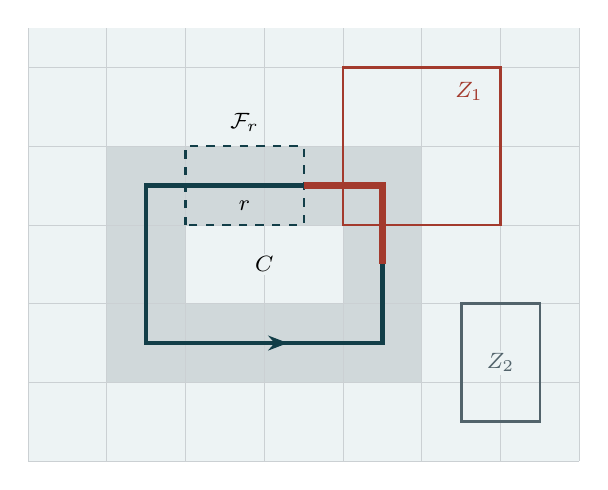
\begin{tikzpicture}[x=5mm, y=5mm,
    lat/.style={draw=muted!30, line width=0.3pt},
    term/.style={draw=ink, line width=1.6pt},
    lab/.style={font=\footnotesize, inner sep=1pt}]

    \fill[pale] (0,0) rectangle (14,11);
    \fill[ink!20, even odd rule] (2,2) rectangle (10,8) (4,4) rectangle (8,6);
    \draw[lat] (0,0) grid (14,11);
    \draw[ink, dashed, line width=0.8pt] (4,6) rectangle (7,8);
    \node[lab, fill=pale] at (5.5,8.6) {$\mathcal F_r$};
    \draw[ink, line width=1.6pt] (3,3) rectangle (9,7);
    \draw[ink, line width=1.6pt, -{Stealth[length=2.5mm]}] (5.5,3) -- (6.6,3);
    \node[lab, fill=ink!20] at (5.5,6.5) {$r$};
    \node[lab, fill=pale] at (6,5) {$C$};
    \draw[markc, line width=2.4pt] (7,7) -- (9,7) -- (9,5);
    \draw[markc, line width=1pt] (8,6) rectangle (12,10);
    \node[lab, fill=pale, text=markc] at (11.2,9.4) {$Z_1$};
    \draw[muted, line width=1pt] (11,1) rectangle (13,4);
    \node[lab, fill=pale, text=muted] at (12,2.5) {$Z_2$};
\end{tikzpicture}
\caption{Marks and contacts. The free bonds $I$ are shaded. The dark band is the union of the link stencils of the loop $C$, and the dashed box is the stencil $\mathcal F_r$ of one contour bond $r$. The polymer $Z_1$ meets the band, so it is marked. Its contacts are the traversals in red, the ones whose stencils meet $Z_1$. The polymer $Z_2$ meets no stencil, so it is unmarked, and its zero-mass measure kills every family containing it.}
\end{figure}

\subhead{Contour Intervals}
The loop is a product of matrices taken in order around $C$, so two polymers touching interlaced positions of the contour cannot be separated. The ratio $(\Xi^{\mathrm f}_\xi)^{[\mathcal A]}/\Xi^{\mathrm f}_\xi$ is expressed as $\exp\bigl(-\sum_{\mathfrak c\text{ hits }\mathcal A}\Phi^{\mathrm v}_\xi(\mathfrak c)\bigr)$, where $\Phi^{\mathrm v}_\xi(\mathfrak c)$ is the Ursell weight of a connected cluster $\mathfrak c$ of polymers. 

Expanding the exponential gives terms that are lists of clusters, each attached to the marked polymers it hits. The \emph{contacts} of a marked polymer are the positions along $C$ whose links read its variables. In each term, V4 joins every cluster to the marked polymers it hits, gives each connected piece the shortest cyclic interval of the contour containing its contacts, and merges pieces whose intervals overlap.

A \emph{group} $W$ is one merged piece: a set $\mathcal A(W)$ of marked polymers, a list of clusters $\mathfrak c_1,\dots,\mathfrak c_k$ each hitting one of them, and an interval $\mathcal H(W)$ that is either short or the whole contour. Its weight is
\begin{equation*}
    w_\xi(W)=\frac{(-1)^k}{k!}\prod_{j=1}^k\Phi^{\mathrm v}_\xi(\mathfrak c_j)\;.
\end{equation*}
Two groups are compatible when their polymers are compatible and their intervals are disjoint, and a group covering the whole contour is compatible with no other group. Then
\begin{equation*}
    F_\xi(0)=\sum_{\mathfrak B\,\mathrm{compatible}}A_\xi(\mathfrak B)\;,\qquad A_\xi(\varnothing)=W_\chi(C;U_\xi(0))\;,
\end{equation*}
where $A_\xi(\mathfrak B)$ is the term above for the marked polymers of the groups in $\mathfrak B$, times their weights $w_\xi(W)$. Each group acts on its own interval of the loop, which is the form Section~\hyperref[summary:10]{10} needs.

\idea{Only polymers that touch the loop contribute, and their order along the loop is kept.}


\chapterpage{10}{Extracting the Scalar inside the Expansion}{V4, Lemma 3.26, ``Schur identity'', and Proposition 3.27, ``joint extraction'', in Section 3.8.}

This section factors a scalar out of $F_\xi(0)$: up to defects, it is a number $S^\circ_{\xi,C}$, which depends only on the loop and the geometry of the branch, times the loop at zero fluctuation, $W_\chi(C;U_\xi(0))$. This scalar is the factor that renormalises the loop, and Sections~\hyperref[summary:11]{11}--\hyperref[summary:16]{16} show $S^\circ_{\xi,C}=\kappa_Ce^{E^\circ_\xi}$, so it carries the perimeter and corner factors $\kappa_C$ of the main theorem.

\subhead{The Reference Data}

The reference data has the identity as its background and zero exterior fluctuations, with the same $\Omega_1$, $I$, hosts $Y$, and cutoffs. Its fine field is $e^{iq_{\id}(a)}$ on $\Omega_1$ and the identity off $\Omega_1$, where $q_{\id}$ is the phase $q_{U_1}$ of Section~\hyperref[summary:6]{6} at $U_1=\id$. Every object of Sections~\hyperref[summary:7]{7}--\hyperref[summary:9]{9} has a reference version, marked $\circ$; these pieces of data need not describe a branch. For a group $W$ let $P^\circ_W(a)$ be the ordered product of the reference links along its interval. Its reference coefficient is
\begin{equation*}
    a_W=w^\circ(W)\int\chi\bigl(P^\circ_W(a)\bigr)\,\dd\Bigl(\bigotimes_{D\in\mathcal A(W)}\widehat\nu^\circ_D\Bigr)(a)\;,
\end{equation*}
where $\mathcal A(W)$ are the marked polymers of $W$ and $w^\circ(W)$ is the weight $w_\xi(W)$ of Section~\hyperref[summary:9]{9} at the reference data.

\subhead{The Schur Identity}
At the identity background, a constant gauge transformation $a\mapsto\operatorname{Ad}_ua$ preserves the reference measures and conjugates every link, so $P^\circ_W(\operatorname{Ad}_ua)=uP^\circ_W(a)u^{-1}$. Since $\chi$ is the normalised character of an irreducible representation, Schur's lemma gives for all $h \in G$
\begin{equation*}
    w^\circ(W)\int\chi\bigl(P^\circ_W(a)h\bigr)\,\dd\Bigl(\bigotimes_{D\in\mathcal A(W)}\widehat\nu^\circ_D\Bigr)(a)=a_W\,\chi(h)\;.
\end{equation*}
The scalar is the reference version of the centred Wilson expectation $F_\xi(0)$ of Section~\hyperref[summary:7]{7}:
\begin{equation*}
    S^\circ_{\xi,C}=\int W_\chi\bigl(C;e^{iq_{\id}(a)}\bigr)\,\dd\nu^\circ_{\xi;0}(a)\;.
\end{equation*}

The expansion of Section~\hyperref[summary:9]{9} writes it as a sum over compatible families $\mathfrak B$, and each term reduces to a product:
\begin{itemize}
    \item A link outside the intervals of $\mathfrak B$ reads none of the integrated variables, so it is $e^{iq_{\id}(0)}=\id$. The loop is therefore $\chi\bigl(P^\circ_{W_1}(a)\cdots P^\circ_{W_m}(a)\bigr)$, with the groups in order around the loop.
    \item The groups have disjoint variables, so the Schur identity integrates them out one at a time. Each step leaves a factor $a_W$, and the last leaves $\chi(\id)=1$.
\end{itemize}
Hence
\begin{equation*}
    S^\circ_{\xi,C}=\sum_{\mathfrak B\,\mathrm{compatible}}\prod_{W\in\mathfrak B}a_W\;.
\end{equation*}

\subhead{The Extraction}
The joint defect compares the actual group terms $A_\xi$ of Section~\hyperref[summary:9]{9} with the reference scalars:
\begin{equation*}
    R_\xi(\mathfrak B)=\sum_{\mathcal S\subseteq\mathfrak B}(-1)^{|\mathfrak B\setminus\mathcal S|}\Bigl(\prod_{W\in\mathfrak B\setminus\mathcal S}a_W\Bigr)A_\xi(\mathcal S)\;,\qquad R_\xi(\varnothing)=W_\chi(C;U_\xi(0))\;.
\end{equation*}
At the reference data every nonempty defect vanishes. Inverting this relation in $F_\xi(0)=\sum_{\mathfrak B}A_\xi(\mathfrak B)$, and adding the exterior response of Section~\hyperref[summary:7]{7}, gives exactly
\begin{equation*}
    \int W_\chi(C;U_\xi(a))\,\dd\nu_{\xi;1}(a)=S^\circ_{\xi,C}\,W_\chi(C;U_\xi(0))+\sum_{\mathfrak B\ne\varnothing}S^{\circ,[\mathfrak B]}_{\xi,C}R_\xi(\mathfrak B)+\mathcal B_\xi\;,
\end{equation*}
where $S^{\circ,[\mathfrak B]}_{\xi,C}$ sums over the families compatible with $\mathfrak B$. If the contour's stencils lie in $I$, then $W_\chi(C;U_\xi(0))=W_\chi(C;U_1)$. The three terms are the leading term, the defect, and the exterior response of the main theorem.

\idea{Gauge invariance at the identity turns each group into a scalar. The leading term is that scalar times the loop at zero fluctuation.}

\chapterpage{11}{The Exact Flat Reference Integral}{V4, Section 4; Appendix A, ``The Flat Covariance''; Appendix C, ``The Local Interaction at the Identity''.}

The flat reference is a specified first-step integral. It includes the nonlinear constraint solution and the residual interaction, even though a Gaussian measure is used as its base. This is the integral from which the perimeter and corner coefficients are extracted.

At the identity background, let $\Delta_1$ be the Hessian of the plaquette action plus the exponential gauge-fixing functional. With the free-to-constrained map $\mathsf C$, V4 defines
\begin{equation*}
    \mathsf H=\mathsf C^*\Delta_1\mathsf C\;,
    \qquad \mathsf K_B=\mathsf H^{-1}\;,
    \qquad \mathsf K=\mathsf C\mathsf K_B\mathsf C^*\;.
\end{equation*}
The Gaussian law $\mu_{\mathsf K_B}$ is on free-bond variables. The reconstructed fine linear field has covariance $\mathsf K$. These are different operators on different carriers. The positive quadratic form includes both the constraint and the stated gauge fixing; no additional zero-mode subtraction is introduced.

The nonlinear reference field is $U_{g_0}=e^{iq_{g_0}(B)}$, where $q_{g_0}(B)=g_0\mathsf CB-h\widetilde D(g_0\mathsf CB)$. The hard cutoff is
\begin{equation*}
    \vartheta_{g_0}(B)
        =\prod_{b\in E_*}\id_{\{|B(b)|<r\}}\;.
\end{equation*}
The same fixed norm and cutoff are used in numerator and denominator.

Let $J_{g_0}$ be the exact constraint-substitution determinant multiplied by the normalised Haar densities of the reconstructed phases. With $\mathscr A$ denoting action plus gauge fixing, the residual exponent is defined by
\begin{equation*}
    \mathcal P_{g_0}(B)=\log J_{g_0}(B)
        -g_0^{-2}\mathscr A(U_{g_0})
        +\frac{1}{2}\langle B,\mathsf HB\rangle\;.
\end{equation*}
The final quadratic term compensates for the Gaussian density. Thus the ratio
\begin{equation*}
    \mathcal W_T^\circ(C)
        =\frac{\int\vartheta_{g_0}(B)e^{\mathcal P_{g_0}(B)}
                W_\chi(C;U_{g_0})\,\dd\mu_{\mathsf K_B}(B)}
            {\int\vartheta_{g_0}(B)e^{\mathcal P_{g_0}(B)}
                \,\dd\mu_{\mathsf K_B}(B)}
        =\frac{N_{C,T}}{D_T}\;,
\end{equation*}
retains the original reference interaction and cutoff. Only scalar prefactors common to this same numerator and denominator have cancelled.

\idea{The Gaussian covariance organises the calculation. It does not replace the nonlinear interacting reference integral by a Gaussian Wilson expectation, and the flat reference law does not replace the physical history law.}

\chapterpage{12}{Gaussian Marginals and Hard Cutoffs}{V4, Section 5, ``Connected Terms'' and ``The Integrated Density Estimate''.}

The flat expansion works with finite principal Gaussian marginals. Appendix A supplies uniform spectral and exponential-decay bounds for the free covariance $C_T=\mathsf K_B$:
\begin{equation*}
    \lambda\id\leqslant  C_T\leqslant  \Lambda\id\;,
    \qquad \|C_T(b,c)\|\leqslant  Ae^{-\mu d_T(b,c)}\;.
\end{equation*}
Here $d_T$ is the periodic bond metric. The constants are independent of the compatible torus. Principal marginal covariances inherit the spectral bounds, so the estimates can be applied on the finite set of inputs of a selected term.

For a local residual $v$ with support $\Lambda_v$, the ordinary and bad-cutoff labels are
\begin{equation*}
    f_v=\left(\prod_{b\in \Lambda_v}\vartheta_b\right)(e^v-1)\;,
    \qquad h_b=-(1-\vartheta_b)\;.
\end{equation*}
The protected cutoffs ensure that $v$ is evaluated only where its chart is defined. Source labels are closed finite differences of the ordered contour word. Expanding these labels gives integrals with bounded, possibly nonsmooth factors.

\subhead{Differentiate the Density}
A hard indicator has no ordinary smooth derivative across its boundary. V4's forest interpolation differentiates covariance parameters in the Gaussian density, leaving the measurable cutoff factors inside the integral. Complex Cauchy estimates then bound those density derivatives.

For a forest edge $e=\{b,c\}$, with vertex degrees $d_b,d_c$, V4 chooses the radius
\begin{equation*}
    r_e=\frac{\lambda}{8d_bd_c\|C_T(b,c)\|}\;.
\end{equation*}
A vanishing covariance block gives a vanishing differentiated term. On the resulting Cauchy circles, the complex covariance $M$ has positive real part. The determinant and the real part of $M^{-1}$ give an integrable Gaussian majorant for the full density. Both are needed: decay of formal covariance coefficients alone would not control the absolute integral of a complex Gaussian.

The resulting integrated bound pays $Cg_0(1+r)^3$ for an ordinary label and $Ce^{-cr^2}$ for a bad bond. A closed source with several selected traversals contributes their small source powers. A single selected traversal has an extra power because $\dd\chi_{\id}=0$. For a component inside a larger word, the corresponding gain is obtained after its exact reference integration and Schur reduction.

The forest degrees generate factors $d_b^{d_b}$. Spatial decay pays them: in four dimensions, many distinct neighbours force a large total distance from the root. A portion of the exponential edge decay absorbs those factors, leaving decay for later support and contour-length estimates.

\idea{The estimate is an integrated density estimate with its normalising determinant retained. It neither differentiates away the hard cutoff nor infers density domination from cancellation.}

\chapterpage{13}{Connected Logarithms and Spatial Decay}{V4, Section 5, especially ``Extent Weights and the Square Geometry''.}

The numerator and denominator of the flat ratio each contain vacuum fluctuations throughout the lattice. Taking their logarithmic difference removes clusters that never touch the source. What remains is a connected expansion localised near the contour, with a quantitative cost for reaching far away.

V4 first assembles the forest components into vacuum objects and source webs. The webs also carry contour intervals, so compatible objects have the required disjointness in space and in the ordered word. The exact gas representation is then converted into a convergent connected logarithm. The logarithm is the branch continued from zero source, where the normalised ratio equals one.

Writing $\Phi_C(\Gamma)$ for a connected source-cluster weight and $J_\Gamma$ for the coarse contour segments containing its source marks, the essential rooted estimate has the form
\begin{equation*}
    \sum_{\substack{\Gamma\\j\in J_\Gamma}}
        |\Phi_C(\Gamma)|e^{\eta\ell(\Gamma)}
        \leqslant  C\tau^2\;.
\end{equation*}
The extent $\ell(\Gamma)$ is the specified network weight of the expansion, including the geometric carrier and interval costs. A fixed positive fraction of its exponential weight survives the counting argument. Constants are independent of the square size and of admitted torus periods.

\subhead{Why the Source Starts at Second Order}
A vacuum component needs only one small label, whereas a source component has at least two small powers: two source marks already provide them, and a single mark receives the additional character cancellation described in Section 12. This leads to source loads of order $\tau^2$, rather than order $\tau$.

The Koteck\'y--Preiss criterion pays incompatible objects with spatial and interval size budgets. The pinned-tree estimate then controls clusters attached to a specified contour segment. This is the quantitative reason that a long straight portion has a finite density per coarse segment.

\subhead{How Geometry Uses the Estimate}
If a cluster joins a root segment to another side of the square, it must have enough extent to bridge that distance. A root far from a corner therefore has an exponentially small contribution to mixed-side terms. Similarly, a cluster that detects a torus image must travel a distance comparable to a period. These observations lead to the separate perimeter, corner, and finite-size terms.

Existence of the reference coefficients uses truncation in extent, convergence of finitely many Gaussian marginal integrals, and removal of the truncation with this rooted tail bound. It does not require constructing an infinite-volume vacuum probability measure or taking a limit of its partition function.

\idea{The connected logarithm turns a multiplicative loop factor into a sum of local source clusters. Exponential extent weights then distinguish a density along an edge from a contribution confined to a corner.}

\chapterpage{14}{The Perimeter Coefficient}{V4, Section 5, ``The Perimeter Coefficient''; equations (5.33) and (5.39).}

Fix one orientation $v$ among $e_1,e_2,-e_1,-e_2$. Consider the infinite reference line in that orientation, divided into segments of $L$ fine traversals. Every finite selected source word is closed by the reverse reference transport. Only finite-dimensional marginal integrals occur in a cluster weight, even though the set of available reference positions is infinite.

For a line cluster $\Gamma$, let $J_\Gamma\subset\mathbb Z$ be the nonempty set of coarse segments containing source marks. V4 allocates its weight equally over those segments and defines
\begin{equation*}
    \kappa_v(g_0)
        =\sum_{\substack{\Gamma\\0\in J_\Gamma}}
            \frac{\Phi_v(\Gamma)}{|J_\Gamma|}\;,
    \qquad
    \delta m_v=-\frac{\kappa_v}{L\varepsilon}\;.
\end{equation*}
The allocation prevents counting one translated connected contribution once for each of its marked segments. Absolute convergence and $|\kappa_v|\leqslant  C\tau^2$ follow from the rooted extent estimate.

If $F_v(m)$ is the connected logarithm of a finite straight relative word of $m$ coarse segments, V4 obtains
\begin{equation*}
    |F_v(m)-m\kappa_v|\leqslant  C\tau^2\;.
\end{equation*}
The bounded difference comes from clusters whose marked set would cross an endpoint of that interval. A cluster rooted far from either endpoint must be long to do so. Summing the resulting exponential tail leaves an endpoint-sized correction, rather than another length-sized term.

For the square, all four orientations enter. The coefficient used in the theorem is
\begin{equation*}
    \delta m(g_0,\varepsilon)
        =-\frac{1}{4L\varepsilon}
            \sum_{v\in \{e_1,e_2,-e_1,-e_2\}}\kappa_v(g_0)\;.
\end{equation*}
The logarithm of the square ratio, divided by $4nL\varepsilon$, tends to $-\delta m$ on the prescribed buffered reference tori. The proof first fixes an extent cutoff, takes the geometric limit, and then removes the cutoff. The bounded corner terms disappear after division by perimeter.

The coefficient is real because reversing a reference line conjugates its character and its connected density: $\kappa_{-v}=\overline{\kappa_v}$. Equality of all four oriented densities is not presumed. Its sign is not determined in V4. The notation ``mass'' therefore identifies a perimeter counterterm; it is not a statement establishing a positive physical mass gap.

\idea{The coefficient is a density per physical length, with the factor $L\varepsilon$ fixed by the coarse-segment convention. It contains the full reference interaction and cutoff dependence.}

\chapterpage{15}{The Corner Coefficient}{V4, Section 6; equations (6.4) and (6.12); local corner subtraction and square identification.}

A corner is the local excess remaining when the densities of its two straight rays have been subtracted. This subtraction must use the same line coefficients already extracted, or it would change the perimeter prescription.

Take perpendicular incoming and outgoing orientations $v,w$. The reference path follows the $v$ ray into the origin and the $w$ ray away from it. Its bend lies between coarse segments $-1$ and $0$. Let $a_{v,w}(j)$ be the rooted connected density at segment $j$, using exactly the same primitives, cutoffs, and Gaussian marginal prescription as for a line.

Define $k_{v,w}(j)=\kappa_v$ on the negative half-line and $k_{v,w}(j)=\kappa_w$ on the nonnegative half-line. V4's local corner logarithm and factor are
\begin{equation*}
    \zeta_{v,w}=\sum_{j\in \mathbb Z}
        \bigl(a_{v,w}(j)-k_{v,w}(j)\bigr)\;,
    \qquad z_{v,w}=e^{\zeta_{v,w}}\;.
\end{equation*}
The cancellation is local in a precise sense. Clusters with source marks entirely on one ray agree with their straight-line counterparts. The surviving differences must have source marks on both sides of the cut, even though vacuum parts of a cluster may extend across it. A root at large $|j|$ must therefore be joined to the other half-line by a long cluster.

The resulting bound is
\begin{equation*}
    |a_{v,w}(j)-k_{v,w}(j)|\leqslant  C\tau^2e^{-c|j|}\;,
    \qquad |\zeta_{v,w}|\leqslant  C\tau^2\;.
\end{equation*}
The sum includes the deficits created by cutting the straight reference words, as well as interactions that join the two perpendicular rays. Keeping only the latter would miss part of the corner constant.

The square has four oriented incoming/outgoing pairs, denoted by $\mathscr C_\square$. V4 defines
\begin{equation*}
    z_{\mathrm c}(g_0,\pi/2)
        =\exp \left(\frac{1}{4}
            \sum_{(v,w)\in \mathscr C_\square}\zeta_{v,w}\right)\;.
\end{equation*}
This fixes the fourth-root branch through the convergent logarithm. It is the geometric mean of the four oriented factors; equality of them is unnecessary. For real-valued characters these corner factors are positive. A general complex character requires no such positivity assertion.

For the infinite-reference square, the remainder after subtracting perimeter and four corner logarithms is bounded by $C\tau^2(n+1)e^{-cn}$. The coefficient is therefore also characterised by taking the bulk torus limit at fixed square, and then taking the large-square constant term. That order of limits belongs to the definition.

\chapterpage{16}{Returning to a Conditional Region}{V4, Section 7; Proposition 7.3; Appendix F, regional scalar identification.}

The line and corner calculations use a translation-invariant reference. The scalar needed by the actual branch expansion is integrated only over a conditional carrier $D$. Its Gaussian covariance is the inverse of the restricted precision,
\begin{equation*}
    C_{D,T}=(i_{D,T}^*H_Ti_{D,T})^{-1}\;.
\end{equation*}
Here $i_{D,T}$ extends a free field by zero to the torus carrier. This operator is generally different from restricting the full covariance $H_T^{-1}$ to $D$. Conditional integration and taking a marginal are different operations.

The regional reference scalar retains all original local labels whose stencils meet $D$, including crossing plaquette and gauge terms. The exterior reference input is zero, while the geometric labels are frozen. This is a reference evaluation of the conditional kernel, not an evaluation of physical large-field indicators at zero field.

Coverage means that $D$ contains every free-input stencil of the contour. Let $K_j$ be the union of those stencils for coarse segment $j$. With $R_0$ the fixed range allowance and $N_{\min }$ the shortest fine period, put
\begin{equation*}
    d_j=\max \bigl(0,d_T(K_j,D^c)-R_0\bigr)\;,
    \qquad \iota_T=\max \bigl(0,N_{\min }/4-R_0\bigr)\;.
\end{equation*}
This $R_0$ is a local range constant of the comparison, distinct from similarly named RG scale parameters. Distance to an empty complement is infinite.

V4 identifies the regional scalar as
\begin{equation*}
    S^\circ_{D,C_n,T}=\kappa_{C_n}e^{E^\circ_{D,C_n,T}}\;,
\end{equation*}
where
\begin{equation*}
    |E^\circ_{D,C_n,T}|\leqslant  C\tau^2
        \left[\sum_{j=0}^{4n-1}e^{-cd_j}
            +4ne^{-c\iota_T}+(n+1)e^{-cn}\right]\;.
\end{equation*}
The three terms have distinct origins. The first compares the restricted kernel and its local summation range with the full torus reference. The second compares the torus with the bulk reference. The third is the distant-corner remainder of the bulk square extraction.

This is the bridge that makes the flat coefficients applicable to a physical branch. Uniform charts identify the two primitive constructions on the actual cutoff box; the covariance and connected-cluster comparisons pay their boundary difference. If a covered contour segment lies close to $D^c$, its $d_j$ can be zero and its contribution is merely $C\tau^2$. Coverage does not imply a large boundary distance.

\idea{The same scalar coefficients survive the regional comparison, but the change of kernel and integration region survives too, as the explicit exponent $E^\circ$.}

\chapterpage{17}{Exterior Response as a Covariance}{V4, Appendix D, Sections D.2--D.5; Lemma D.6.}

The exterior response compares the actual conditional law with its centred version. Its operand is the covariance of the full Wilson character with the interpolation score, under the actual normalised conditional law. This retains the nonlinear residual interaction and the physical hard cutoff.

The regular-background estimates give a positive lower bound $\gamma\id\leqslant  H$ for the conditional precision. The local primitive bounds make the Hessian of the residual perturbation small compared with $\gamma$. Consequently the real conditional potential remains uniformly convex on the admitted domain. Locality also bounds its off-diagonal Hessian entries and their range.

\subhead{Keeping the Hard Boundary}
The integration domain is a product of convex norm balls. V4 extends the functions within a proved enlarged chart and approximates the hard domain by smooth convex barriers. Each barrier is a sum of single-bond functions, so its Hessian is diagonal in the bond labels. Its large diagonal contribution preserves convexity without worsening the off-diagonal decay constants.

For real test functions $u,v$ in the stated weighted $H^1$ space, the smooth barrier law has the Helffer--Sj\"ostrand identity below. V4 denotes its one-form operator by $\mathscr A_{n,t}$ and obtains the spatial inverse estimate alongside it:
\begin{equation*}
    \operatorname{Cov}_{\nu_{n,t}}(u,v)
        =\langle\nabla u,\mathscr A_{n,t}^{-1}\nabla v\rangle\;,
    \qquad
    \|\Pi_b\mathscr A_{n,t}^{-1}\Pi_c\|
        \leqslant  \frac{4}{\gamma}e^{-\mu d(b,c)}\;.
\end{equation*}
Here $n$ is the barrier index, unrelated to the square size in this local argument. The inverse estimate follows from a spatial exponential weight and the off-diagonal Hessian bounds. The complex Wilson function is handled through its real and imaginary parts. Passing to the barrier limit returns the original normalised hard-box law.

The Wilson gradient is supported on the contour's free-input set $I_C$. The score gradient is supported in a fixed shell next to the exterior carrier $J$. The covariance estimate therefore yields, on covered branches,
\begin{equation*}
    |\mathcal B_\xi[f_\xi]|
        \leqslant  C_{\mathrm{resp},\chi}g_0rD_\xi\;,
    \qquad D_\xi=\sum_{b\in I_C}e^{-\mu d(b,J)/2}\;.
\end{equation*}
If $J$ is empty, the score and this bound vanish. The constants do not depend on the branch, the volume, the interpolation parameter, or the barrier index.

An integration-by-parts expression for the same response contains two hard-cutoff flux terms, including the flux from the normaliser. V4's covariance argument bounds the whole expression. It does not declare either surface term to be zero or discard it after shifting the Gaussian.

\idea{The boundary is handled by convexity and a limit back to the same conditional law. A covariance estimate for an uncut Gaussian would not supply this result.}

\chapterpage{18}{Paying Bad Regions with Physical Witnesses}{V4, Appendix D, especially one-point witnesses, the retained physical normaliser, and Proposition D.15.}

The conditional response bound is useful only after averaging over histories. Some branches have a bad region near the contour, and some are not covered at all. Their rarity must be measured under the physical law, rather than under a fresh Gaussian law assigned to frozen exterior coordinates.

V4 traces a bond in the filled bad region to a nearby failed cutoff. The failure supplies a witness: either a plaquette holonomy or an auxiliary gauge variable exceeds a specified threshold. Filling can enlarge the bad region, but its construction keeps a bad point within a controlled macroscopic distance. The number of possible local witness labels is explicitly counted.

Reversing the exact changes of variables and the partitions of unity returns the marked integral to the original Wilson measure, with the auxiliary gauge integrals retained. The physical normaliser is still $\mathcal Z_0$. A lower bound on that same partition function is part of the witness-tail argument. It is not an alternative normalisation of the histories.

For a positive bond $z$, write $p_z$ for the physical probability that it meets the filled bad region. The one-point estimate is
\begin{equation*}
    p_z\leqslant  q\leqslant  e^{-c_*\pi_*^2}\;.
\end{equation*}
The plaquette part uses reflection positivity and a chessboard estimate on the admitted even tori. An action cost for a disseminated bad plaquette is compared with the physical partition function lower bound. The gauge-variable part uses its own normalised auxiliary measure. The final union bound includes the possible witness locations.

This produces the history estimates needed for the original carrier:
\begin{equation*}
    \Ph(A_{\mathrm{cov}}^c)\leqslant  C_Ln_Cq\;,
    \qquad \Eh[\id_{A_{\mathrm{cov}}}D_\xi]\leqslant  Cn_Cq\;.
\end{equation*}
The contour and its reconstruction stencils contain only a fixed multiple of $n_C$ bonds. Exponential distance weights have a volume-independent lattice sum, which explains the retained perimeter factor.

The boundary error is exactly the covered response plus the uncovered conditional expectation,
\begin{equation*}
    E_{\mathrm{bdry}}=\Eh\!\left[
        \id_{A_{\mathrm{cov}}}\mathcal B_\xi[f_\xi]
            +\id_{A_{\mathrm{cov}}^c}F_\xi(1)\right]\;.
\end{equation*}
Using $|F_\xi(1)|\leqslant  1$ and the response bound gives the main theorem's estimate $C_{\mathrm{resp},\chi}n_C(1+g_0r)e^{-c_*\pi_*^2}$.

\idea{The marks are correlated under the history law. One-point bounds suffice for these linear sums, but do not alone imply the joint estimates needed for an exponential moment.}

\chapterpage{19}{The Signed Integrated Defect}{V4, Appendix E; Proposition E.22, equations (E.78)--(E.79).}

The defect operand is the signed family sum from scalar extraction, averaged with the original branch weight:
\begin{equation*}
    \mathscr R_\xi
        =\sum_{\varnothing\ne \mathfrak B\,\mathrm{compatible}}
            S^{\circ,[\mathfrak B]}_{\xi,C}R_\xi(\mathfrak B)\;,
    \qquad
    E_{\mathrm{def}}=\Eh[\id_{A_{\mathrm{cov}}}\mathscr R_\xi]\;.
\end{equation*}
V4 splits histories according to whether the filled bad region lies within distance $b=\lfloor LMR_1/16\rfloor$ of the contour's input templates. This is a decomposition of an expectation under the same law.

On near histories, the whole signed sum satisfies $|\mathscr R_\xi|\leqslant  2$. Indeed, it equals the difference between two normalised closed-character expressions of modulus at most one. This bound is used after summing the joint defects; it is not a uniform small bound on every individual group term. One-point witnesses then give the absolute near-history contribution $C'_Ln_Ce^{-(c_*/2)\pi_*^2}$.

\subhead{The Additional Gain on Far Histories}
For far histories, the proof returns to signed selected integrals. Zero-mass probes act as finite differences inside a closed character. Odd leading terms cancel against the even Gaussian/cutoff kernel. Ordinary interaction factors disturb that symmetry; an independent complex parameter on each root pays their contribution by a Cauchy estimate. The resulting gain per marked root is
\begin{equation*}
    \rho=O\bigl(g_0^2(1+r)^4\bigr)\;.
\end{equation*}
Total-variation majorants enter only after these cancellations. A single background derivative then compares a closed group with its flat reference. The comparison includes the background transports along its contour interval and its closing word, not just its random-field support. Local curvature bounds pay small interior groups; extent decay pays large groups or groups reaching the bad region.

The positive group sum retains one joint reference exclusion ratio and yields, on covered far histories,
\begin{equation*}
    |\mathscr R_\xi|
        \leqslant  |S^\circ_{\xi,C}|(e^x-1)\;,
    \qquad x=C_\chi n_C\rho
        \bigl(\varepsilon_1+e^{-cb/(LM)}\bigr)\;.
\end{equation*}
After physical averaging, this is stronger than discarding $|S^\circ_{\xi,C}|\leqslant  1$. Substituting $S^\circ_{\xi,C}=\kappa_Ce^{E^\circ_\xi}$ retains a factor $|\kappa_C|$, paid together with the exponential moment of $E^\circ_\xi$. The near-history part remains absolute.

\idea{The far defect is relative to a regional reference scalar before averaging. The exponential $e^x-1$ is small only in a regime controlling $x$; its exponent cannot be silently replaced by a linear error for arbitrary contour length.}

\chapterpage{20}{Why the Integration Region Retreats}{V4, Section 9.1--9.4; the mean shift, physical collar payment and termination lemmas.}

The quadratic coupling to exterior free variables gives a conditional mean
\begin{equation*}
    m=-H_{DD}^{-1}H_{DJ}A'_{\mathrm e}\;,
    \qquad D=I\;,
\end{equation*}
where $A'_{\mathrm e}$ is the exterior input after the boundary change. Exponential decay of $H_{DD}^{-1}$ controls the shift away from the collar. Close to the boundary, a large exterior coordinate can still move the conditional Gaussian towards the edge of the hard integration box.

V4 inserts a second cutoff test on the exterior collar: a collar bond is good when $|A_{\mathrm e}(e)|<\vartheta r$, with a fixed sufficiently small $\vartheta$. The test is a partition of unity inside the original integrand. It introduces labels, rather than conditioning the whole law on every collar bond being good.

\subhead{The Retreat Procedure}
The inner region is first filled according to the stated rectangular-hull rule. At each later round, a failed collar test removes the nearby macroscopic cubes; the region is filled again. In the source's notation, the update is
\begin{equation*}
    \Lambda_1^{(k+1)}
        =\operatorname{Fill}\left(
            \Lambda_1^{(k)}\setminus
                \bigcup_{e\in B^{(k)}}\mathcal Q(e)\right)\;.
\end{equation*}
The set $B^{(k)}$ lists the newly bad collar bonds, and $\mathcal Q(e)$ is the prescribed neighbourhood in macroscopic cubes. A nonterminal round removes at least one cube, so the finite-volume procedure terminates. The terminal collar is good, and its mean shift satisfies $\|m\|_\infty\leqslant  r/4$. This leaves the margin needed for translated-box estimates.

The coordinates removed from the integrated carrier become exterior coordinates of that labelled term. Their old good-box factors remain in the integrand. The underlying fine field, its background, the boundary change, its Jacobian, and the original interaction are unchanged. The procedure changes the order and split of the integrations, with the inherited conditional law retained.

With $\ell=LMR_1$, a bond removed after the initial filling is attributed to a bad collar bond within the source's fixed distance allowance. The multiplicity is bounded by $N_{\mathrm{ret}}=4(207\ell)^4$. Physical witness probabilities pay that multiplicity. The argument does not assume a convenient lower bound for an exterior Schur-complement density.

\idea{Retreat creates a safe conditional integration region on each labelled term. It does not delete a bad physical event or replace the original distribution by a newly chosen exterior Gaussian.}

\chapterpage{21}{Labelled Sums and the Second-Order Rate}{V4, Sections 9.5--9.9; Proposition 9.34; boundary accounting and labelled defects.}

After retreat, the leading scalar must be identified at the terminal carrier $D(\Lambda)$ itself. It is not enough to remove the groups that visibly touch the deleted bonds: restricting the carrier changes the reference precision, eligible probe labels, selected marginal covariances, and local activities. V4 applies the regional comparison again and obtains $S^\circ_\Lambda=\kappa_Ce^{E^\circ_\Lambda}$.

The labelled weights form an exact positive partition of the original weight,
\begin{equation*}
    \sum_{\mathrm{lab}}\mathsf w^{\mathrm{lab}}_\xi
        =\mathsf w_\xi\;.
\end{equation*}
Integrations over removed inner coordinates are included in $\mathsf w^{\mathrm{lab}}_\xi$. Thus the labelled physical average has the same normaliser $\mathcal Z_0$.

One-point accounting now sees two sources of bad bonds: the original filled bad region and the failures that cause retreat. The resulting cost is of the form $q+N_{\mathrm{ret}}q_\vartheta$, with $q_\vartheta\leqslant  e^{-c_q\vartheta^2\pi_*^2}$. Coverage failures and weighted exterior sums are paid by this cost. Polynomial collar and cutoff factors can be absorbed into part of the witness exponent at small coupling.

\subhead{The Cost of Summing Undifferenced Groups}
The source-containing boundary estimate sums families with a marked, differenced slot and other slots that remain undifferenced. A first estimate pays the latter at a first-order rate. V4's second-order refinement reuses the even-kernel and interaction-parameter mechanisms on those undifferenced closed contractions. The improved family factor is
\begin{equation*}
    e^{n_C\bar\varepsilon_{\mathrm{ph}}}\;,
    \qquad
    \bar\varepsilon_{\mathrm{ph}}
        =O\bigl(g_0^2(1+r)^4\bigr)=O(\tau^2)\;.
\end{equation*}
The first-order quantity survives in a prefactor attached to the marked exterior term, rather than in that exponent. The distinction matters because an undifferenced slot can occur anywhere along the contour.

The labelled signed defect has the same near/far structure as at the original carrier. Its far part retains $|S^\circ_\Lambda|$ and becomes relative after scalar identification and moment control; its near part is an absolute rare-history contribution. These are bounds on a resplitting of the first-step integral, not a second RG transformation.

The second-order rate is quantitatively better, but its factor still grows with $n_C$ at fixed coupling. V4 explicitly records that a bound uniform in contour length would require resumming the undifferenced slots against the reference exclusions. That resummation is not contained in the stated result.

\idea{Improving a per-bond rate from first to second order is useful. It does not make an exponential family sum independent of the number of bonds.}

\chapterpage{22}{Averaging the Finite-Geometry Exponent}{V4, Corollary 1.4; Section 9, joint witnesses and exponential moments.}

The pointwise bound on $E^\circ_\xi$ contains one possible boundary contribution per coarse segment. A small first moment of that sum would not, by itself, control its exponential. V4 therefore proves joint witness estimates and an exponential-moment bound under the physical history law.

At the original carrier, the exponent splits as
\begin{equation*}
    E^\circ_\xi=E^\partial_\xi+E^\circ_{T,n}\;.
\end{equation*}
The carrier part $E^\partial_\xi=F_{I,C,T}-F_{C,T}$ is history-dependent. The remainder $E^\circ_{T,n}$ contains the torus-to-bulk and distant-corner terms and is deterministic at fixed reference parameters. Its exact scalar identification is $\kappa_Ce^{E^\circ_{T,n}}=\mathcal W_T^\circ(C_n)$.

Under the additional torus condition $4ne^{-c\iota_T}\leqslant  1$, V4 obtains
\begin{equation*}
    |E^\circ_{T,n}|\leqslant  C\tau^2(2+1/c)\;,
    \qquad
    \Eh[\id_{A_{\mathrm{cov}}}e^{|E^\circ_\xi|}]
        \leqslant  e^{C\tau^2(2+1/c)+n_C\delta^\sharp_q}\;.
\end{equation*}
The original-carrier rate in Corollary 1.4 is
\begin{equation*}
    \delta^\sharp_q
        =C\tau^2N'_{\mathrm{lat}}(c)
            e^{C\tau^2L^4C_K\Phi_c}q^{1/16}\;.
\end{equation*}
Here $N'_{\mathrm{lat}}(c)$ is a finite lattice shell sum and $\Phi_c$ bounds the exponentially weighted contour load at one bond. Both are independent of contour length and coupling. The witness neighbourhood count $C_K=4(4K\ell+9)^4$, with $K=256$ and $\ell=LMR_1$, does depend on coupling. At the further small-coupling threshold, the exponential factor is at most $e$, and the rate is bounded by $eC\tau^2N'_{\mathrm{lat}}(c)e^{-c_q\pi_*^2/16}$.

The fixed fraction $1/16$ comes from dividing four-dimensional boxes into sixteen separated classes and applying the joint witness bound to separated representatives. It is not independence of all bad-region marks. The labelled, retreated construction has its own stated moment estimate; the strengthened rate displayed here belongs to the original carrier.

Corollary 1.4 then writes the leading term exactly as
\begin{equation*}
    \begin{aligned}
        \kappa_C\Eh[\id_{A_{\mathrm{cov}}}e^{E^\circ_\xi}W_\chi(C_n;U_1)]
        &=\mathcal W_T^\circ(C_n)
            \bigl(\Eh[\id_{A_{\mathrm{cov}}}W_\chi(C_n;U_1)]+R_n\bigr)\;,\\
        |R_n|&\leqslant  e^{n_C\delta^\sharp_q}-1\;.
    \end{aligned}
\end{equation*}
Thus the deterministic reference geometry can be separated from the physical background loop. The remaining error is still a perimeter-rate error, despite its very small rate.

\chapterpage{23}{The Size of the Leading Term at a Fixed Loop}{V4, Corollary 1.5; Remark 1.3, on the regime, following Theorem 1.2.}

A nonzero extracted scalar does not ensure a nonzero retained expectation: a complex character can cancel in an average. V4 supplies a separate small-coupling estimate for each fixed lattice square.

On the event that the whole square surface lies in the regular region, each of its plaquette holonomies is close to the identity. V4's lattice Stokes argument assembles them in their nonabelian order, with the necessary conjugations. Unitarity bounds the deviation of the resulting closed holonomy by the sum of plaquette deviations. The failure of this surface event is paid by a one-point union bound.

Let $\mathrm{Lip}_\chi$ be the stated Lipschitz constant of the representation, and $c_{\mathrm h}=\sqrt N$. With $n_C=4nL$, the source gives
\begin{equation*}
    \begin{aligned}
        \left|\Eh[\id_{A_{\mathrm{cov}}}W_\chi(C_n;U_1)]-1\right|
        &\leqslant  a_n\;,\\
        a_n&=2\mathrm{Lip}_\chi c_{\mathrm h}(nL)^2\varepsilon_1
            +\bigl(2(nL+1)^2+C_Ln_C\bigr)q\;.
    \end{aligned}
\end{equation*}
Combining this with the factorisation of Section 22 yields
\begin{equation*}
    \begin{aligned}
        \kappa_C\Eh[\id_{A_{\mathrm{cov}}}e^{E^\circ_\xi}W_\chi(C_n;U_1)]
            &=\mathcal W_T^\circ(C_n)(1+R_n^\sharp)\;,\\
        |R_n^\sharp|&\leqslant  \eta_n
            :=a_n+e^{n_C\delta^\sharp_q}-1\;.
    \end{aligned}
\end{equation*}
When $\eta_n<1$, the leading term is nonzero. Its modulus lies between $(1-\eta_n)|\mathcal W_T^\circ(C_n)|$ and $(1+\eta_n)|\mathcal W_T^\circ(C_n)|$. The deterministic geometry bound also compares the reference factor with $|\kappa_C|$ up to $e^{\pm C\tau^2(2+1/c)}$.

For each fixed $n$, the source states $\eta_n\to0$ as $g_0\to0$, on tori satisfying the coupling-dependent hypotheses. The controlling background term has an area factor $(nL)^2\varepsilon_1$. The estimate is small for loops whose lattice side is at most a sufficiently small multiple of $\varepsilon_1^{-1/2}$; it is not uniform in $n$.

This matters even at the conjectured final plaquette. At $n=1$, the background estimate contains $L^2\varepsilon_1$, which is not of order $\tau^2$ in the stated small-coupling regime. V4 therefore does not deduce the endpoint precision required by its iteration conjecture from Corollary 1.5 alone.

\idea{A fixed lattice loop becoming close to the identity at small coupling is a different regime from a fixed physical loop whose number of lattice bonds grows as the cutoff is removed.}

\chapterpage{24}{The Outgoing Insertion and Closed Flux Factors}{V4, Section 8, especially the closed flux insertion and the outgoing measure pair.}

The leading loop in the theorem is $W_\chi(C;U_1)$. The block constraint fixes an average of transports, so it does not generally equate a straight fine transport with the corresponding coarse link.

On a positive covered coarse bond $c$, the regular average has the form $M(U_1,c)=e^{i\beta_c(U_1)}P_c(U_1)=V(c)$. V4 consequently defines
\begin{equation*}
    Y_c=e^{-i\beta_c(U_1)}\;,
    \qquad P_c(U_1)=Y_cV(c)\;.
\end{equation*}
The logarithms entering $\beta_c$ are closed relative transports within the two endpoint blocks. The reversal convention is $Y_{c^{-1}}=V(c)^{-1}Y_c^{-1}V(c)$, which preserves the ordered transport identity.

For the coarse contour $\bar C=(c_1,\ldots,c_m)$, the retained insertion is
\begin{equation*}
    \mathcal L_\xi(C;V)
        =\chi\bigl(Y_{c_1}V(c_1)\cdots Y_{c_m}V(c_m)\bigr)
        =W_\chi(C;U_1)\;.
\end{equation*}
The $Y_c$ factors transform by conjugation at their initial sites, while coarse links transform at their endpoints. Their ordered closed character is gauge invariant. V4 assigns no separate activity norm to a $Y_c$ factor or an open transport.

\subhead{The Other Source Terms Are Retained}
On covered branches define $\mathcal L^{(0)}_\xi=\kappa_Ce^{E^\circ_\xi}\mathcal L_\xi$, and set it to zero on uncovered branches. The exact conditional correction is
\begin{equation*}
    \mathcal H_\xi
        =\frac{\int\bigl[W_\chi(C;U_\xi(a))
                -\mathcal L^{(0)}_\xi\bigr]\mathcal K_\xi(a)\,\dd a}
            {\mathcal J_\xi[1]}\;.
\end{equation*}
This is a definition with the same conditional law and denominator. The manuscript bounds its physical history average through the defect and boundary terms. Here it asserts only the stated trivial pointwise bound on $\mathcal H_\xi$, rather than pointwise smallness and locality in $V$.

After disintegrating the outer branch measure at fixed $V$, the exact $W_1(C;V)$ is the corresponding weighted average of $\mathcal L^{(0)}_\xi+\mathcal H_\xi$. The scalar-extracted outgoing data is the pair
\begin{equation*}
    \bigl(\kappa_C^{-1}N_1,\rho_1\bigr)\;.
\end{equation*}
These measures can be pushed forward again. An iterative analytic theorem additionally needs a closed class of local gauge-invariant insertions and estimates for their transformed activities. A measure-theoretic next step alone does not establish that closure.

\idea{The dressed insertion retains the closed flux factors and the dependence on exterior fields and region choices. V4's comparison pays for every contour bond; the programme is to retain the dressing until the final coarse scale.}

\chapterpage{25}{Two Disjoint Square Loops}{V4, Theorem 1.8, equations (1.18)--(1.20); Section 10, especially the cross-term estimates (10.1) and (10.5).}

V4 extends the calculation to two squares $C_1,C_2$ in planes parallel to the same coordinate plane. They may have different sizes and characters $\chi_1,\chi_2$, but their vertex sets must be disjoint. The observable is the product $W_{12}(U):=W_{\chi_1}(C_1;U)W_{\chi_2}(C_2;U)$, and $n_C=n_{C_1}+n_{C_2}$ counts traversals on both loops. Both use the same background, conditional carrier, and history law. Their geometric disjointness does not make their fluctuations independent.

\subhead{Keep Each Loop's Renormalisation and Isolate Connections}
Under the two-loop theorem's hypotheses, the decomposition is
\begin{equation*}
    \begin{aligned}
        \mathbb E_\varepsilon[W_{12}]
        &=\kappa_{C_1}\kappa_{C_2}\,
            \Eh\!\left[\id_{A_{\mathrm{cov}}}
                e^{E^\circ_{\xi,1}+E^\circ_{\xi,2}+E^\times_\xi}
                W_{12}(U_1)\right]\\
        &\quad+E_{\mathrm{def}}+E_{\mathrm{bdry}}\;.
    \end{aligned}
\end{equation*}
Each $\kappa_{C_i}$ is exactly its single-square factor, with the character of that square. Coverage is required for both loops. The new exponent $E^\times_\xi$ measures the failure of the pair's reference group gas to factor into the two single-square gases.

The marked expansion distinguishes groups belonging to one loop from groups connecting both. Single-loop groups admit the previous Schur extraction. V4 assigns zero scalar coefficient to a connecting group and retains its closed two-loop contraction in the defect. Such a contribution can survive at the identity background: it must be bounded by its spatial extent, rather than by a curvature factor. Thus the pair's reference group gas is not the full normalised flat two-loop integral. Exclusions between the remaining groups also contribute to $E^\times_\xi$.

\subhead{Why Separation Makes the Additional Contributions Small}
For a traversal $a$, let $\delta_a$ be the periodic fine-lattice distance of its initial vertex from the other loop, and let $d=\min_a\delta_a$. V4 uses
\begin{equation*}
    \Delta_\times=\sum_{a\in\mathcal I_{C_1}\sqcup\mathcal I_{C_2}}
        e^{-c_\times\delta_a/(LM)}\;,
    \qquad |E^\times_\xi|\leqslant  C_\times\rho\Delta_\times
        \leqslant  C_\times\rho n_Ce^{-c_\times d/(LM)}\;.
\end{equation*}
A connected contribution joining the loops must span their separation. The existing extent decay pays that distance. This gain is of order $\rho$, with no additional curvature factor for a connecting group.

To read the error bounds, set $x=C_\times\rho\Delta_\times$ and $X=C_\chi n_C\rho(\varepsilon_1+e^{-cb/(LM)})$. Then
\begin{equation*}
    \begin{aligned}
        |E_{\mathrm{def}}|&\leqslant  e^x
            \left[C'_Ln_Ce^{-(c_*/2)\pi_*^2}+e^{X+x}-1\right]\;,\\
        |E_{\mathrm{bdry}}|&\leqslant  C_{\mathrm{resp},\chi_1\chi_2}
            n_C(1+g_0r)e^{-c_*\pi_*^2}\;.
    \end{aligned}
\end{equation*}
The theorem also bounds the joint history moment of the two regional exponents. Its constants are uniform in the loop sizes and positions, with their dependence retained through $n_C$ and $\Delta_\times$. No separation assumption beyond disjoint vertices is imposed; small cross corrections require $x$ small. This controls connections created in the first fluctuation integration. The retained background expectation is still joint, so the result does not assert factorisation of the full loop expectations or a mass gap.

\chapterpage{26}{What Iteration Would Still Require}{V4, Section 11, Conjecture 11.1 and Remark 11.2.}

For $n=L^k$, the square becomes a single plaquette after $k+1$ blocking steps. V4 conjectures coefficients $\delta m_j$ and $z_j=e^{\zeta_j}$, with the first-step values fixed by the construction already described, such that
\begin{equation*}
    \begin{gathered}
        \mathbb E_\varepsilon[W_\chi(C_n)] = \kappa^{(k+1)}_{C_n}(1+R)+R'\;,\\
        \kappa^{(k+1)}_{C_n} = \exp \left(-P(C_n)\sum_{j=1}^{k+1}\delta m_j\right) \prod_{j=1}^{k+1}z_j^4 \; , \\
        |R|\leqslant C\bigl[(k+2)\tau^2+n_Ce^{-c\pi_*^2}\bigr] \; , \qquad |R'|\leqslant Cn_Ce^{-c\pi_*^2} \; .
    \end{gathered}
\end{equation*}
The conjecture uses the first-step scales $\tau$ and $\pi_*$ and allows a small-coupling threshold depending on $k$, with compatible sufficiently large tori. Those quantifiers are part of its scope. The coefficients for $j \geqslant 2$ are not defined by V4's first-step formulas alone.

The source identifies several missing bridges:
\begin{itemize}
    \item \textbf{A local outgoing class.} The reconstructed-background loop, its carrier correction, and remaining source terms must be represented in a form accepted by the next step, with their dependence on coarse fields and history labels controlled.
    \item \textbf{The inherited interaction.} Later steps act on the density already produced, including earlier interactions and the terms introduced by the $\mathbf R$-operations. First-step branch identities do not automatically supply their general-step counterparts.
    \item \textbf{Perimeter-local error extraction.} The far defect and the family factors must be organised as local corrections when a threshold independent of the number of steps is sought. Their present estimates contain exponentials of contour length.
    \item \textbf{An endpoint estimate.} The final retained plaquette expectation needs the conjectured $O(\tau^2)$ precision. The proved fixed-loop estimate still contains an $O(\varepsilon_1)$ area contribution at a plaquette.
\end{itemize}

The absolute boundary and near-history errors also need accounting with the scalar factors of preceding steps. The history-moment remainder and the deterministic torus/corner exponent must be accumulated at each scale with their actual rates. Neither repeated application of an absolute error bound nor a first-step reference coefficient supplies that accounting by itself.

The precision of the conjecture has a further limitation stated in V4: corner factors of size $1+O(\tau^2)$ can be absorbed into its allowed $O((k+2)\tau^2)$ remainder. Thus that remainder alone would not identify higher-step corner coefficients separately. Their definitions would have to come from a construction at each scale.

\idea{V4 gives the first-step architecture and coefficients for one square, together with an extension to two disjoint squares. Its final section states the additional local, inherited-measure, and endpoint work needed for iteration; it does not claim that work is already complete.}

\chapterpage{27}{Source Guide and Essential Distinctions}{How to return from this companion to the current manuscript.}

\subhead{Where to Read Next}
\begin{small}
\begin{tabularx}{\textwidth}{@{}p{0.29\textwidth}X@{}}
    \toprule
    \textbf{Question} & \textbf{Location in V4}\\
    \midrule
    Exact statements and scope & Section 1: Theorems 1.2 and 1.8, Corollaries 1.4 and 1.5, and the regime remarks.\\[3pt]
    Why extract local scalars? & Section 2: comparison with effective-interaction extraction.\\[3pt]
    What is the conditional law? & Section 3: branches, reconstruction, the exact boundary change, polymer and probe measures, joint extraction.\\[3pt]
    Which reference integral? & Section 4; Appendix A for covariance; Appendix C for the local identity-background interaction.\\[3pt]
    How are coefficients defined? & Sections 5--6: line density, local corner subtraction, and the ordered reference limits.\\[3pt]
    Why do they apply regionally? & Section 7, especially Proposition 7.3; Appendix F for the scalar in the physical branch identity.\\[3pt]
    What survives the step? & Section 8: reconstructed loop, closed flux factors, conditional correction, and outgoing measure pair.\\[3pt]
    How are errors controlled? & Appendix D: exterior response and physical witnesses. Appendix E: signed defects and their physical caller.\\[3pt]
    Why add labels and retreat? & Section 9: collar tests, terminal carrier, translated estimates, second-order rate, and history moments.\\[3pt]
    What changes for two loops? & Theorem 1.8 and Section 10: joint extraction, connecting groups, separation decay, and the pair at the retreated carrier.\\[3pt]
    What remains for iteration? & Section 11: Conjecture 11.1 and its explicit list of missing inputs.\\
    \bottomrule
\end{tabularx}
\end{small}

\subhead{Five Distinctions to Keep}
\begin{enumerate}
    \item The free covariance, reconstructed fine covariance, and inverse restricted precision live on different carriers and play different roles.
    \item A reference scalar is extracted with physical history weights left intact; flat evaluation does not set a large-field indicator to its flat value.
    \item Source cancellation is used inside closed signed contractions before absolute majorants are introduced.
    \item An absolute error, a relative error, and a small rate per contour bond have different implications for a long loop.
    \item A fixed-cutoff first step, a fixed lattice loop at small coupling, and an all-scale limit of a fixed physical loop have different quantifiers.
\end{enumerate}

\subhead{Source Snapshot}
The base V4 snapshot is from 22 October 2026; Sections~3 and~24 also use the 23 October revision. Their SHA-256 hashes are:

\begin{footnotesize}
\begin{tabular}{@{}ll@{}}
    22 October & \texttt{D463C554B76FB249EB9D65CD12BB105AF4CE5BC3A76299135EB4317C73094E00}\\
    23 October & \texttt{1EBF0AFE6A24FF420DAE26DDD78A31503BC7E28CD5AF652195F875EE60DE79BD}\\
\end{tabular}
\end{footnotesize}

\begin{thebibliography}{9}
    \bibitem{BalabanRG1}
    T.~Ba{\l}aban,
    \emph{Renormalization Group Approach to Lattice Gauge Field Theories.~I. Generation of Effective Actions in a Small Field Approximation and a Coupling Constant Renormalization in Four Dimensions},
    Commun. Math. Phys. \textbf{109} (1987), 249--301.

    \bibitem{BalabanCRE}
    T.~Ba{\l}aban,
    \emph{Convergent Renormalization Expansions for Lattice Gauge Theories},
    Commun. Math. Phys. \textbf{119} (1988), 243--285.

    \bibitem{BalabanRG2}
    T.~Ba{\l}aban,
    \emph{Renormalization Group Approach to Lattice Gauge Field Theories.~II. Cluster Expansions},
    Commun. Math. Phys. \textbf{116} (1988), 1--22.

    \bibitem{KoteckyPreiss}
    R.~Koteck\'y and D.~Preiss,
    \emph{Cluster Expansion for Abstract Polymer Models},
    Commun. Math. Phys. \textbf{103} (1986), 491--498.
\end{thebibliography}
\end{document}
